%% ═══════════════════════════════════════════════════════════════════════════
\subsection{Methodology: The Agile Test-and-Learn Program}
%% ═══════════════════════════════════════════════════════════════════════════

This R\&D operation is structured as an agile Test-and-Learn program designed to investigate cognitive biases in supply chain urgency assessment and formulate a digital-twin-based correction loop. Rather than following a rigid sequential path, the program operates through continuous iterations of literature analysis, mathematical specification, software implementation, and scenario-based simulation.

The R\&D pipeline is organized into four core operational areas:
\begin{itemize}
    \item \textbf{Literature Review and Gap Analysis}: Establishing the psychological and mathematical foundations of multi-block urgency aggregation and cognitive bias (detailed in Section~\ref{sec:SOTA}).
    \item \textbf{Mathematical Framework Specification}: Deriving and formalizing the multi-block real urgency function, its DAG propagation, and the asymmetric cognitive adequacy score from first principles to ensure dimensional and probabilistic consistency.
    \item \textbf{Pairwise comparison elicitation}: Formulating crisp Analytic Hierarchy Process (AHP) and Fuzzy Best-Worst Method (F-BWM) eigenvectors to build a reliable representation of declared operator urgency.
    \item \textbf{Implementation, Simulation and Validation}: Building a modular, tested Python library (73 modules, 1\,831 automated test functions expanding to 2\,044 collected cases) exercised through a multi-page Dash web application, running controlled shock and scenario simulations on a persistent digital twin, and confronting the hidden-risk signal with recorded outcomes through a dedicated calibration service and a serious-game campaign (Section~\ref{sec:serious_game}).
\end{itemize}

The remainder of this section follows that same separation explicitly: the mathematical model is presented on its own (Section~\ref{sec:math_framework}), independently of how it is elicited, computed, and exposed (Section~\ref{sec:application}), before turning to the use case built to validate it (Section~\ref{sec:serious_game}).

\begin{figure}[H]
    \centering
    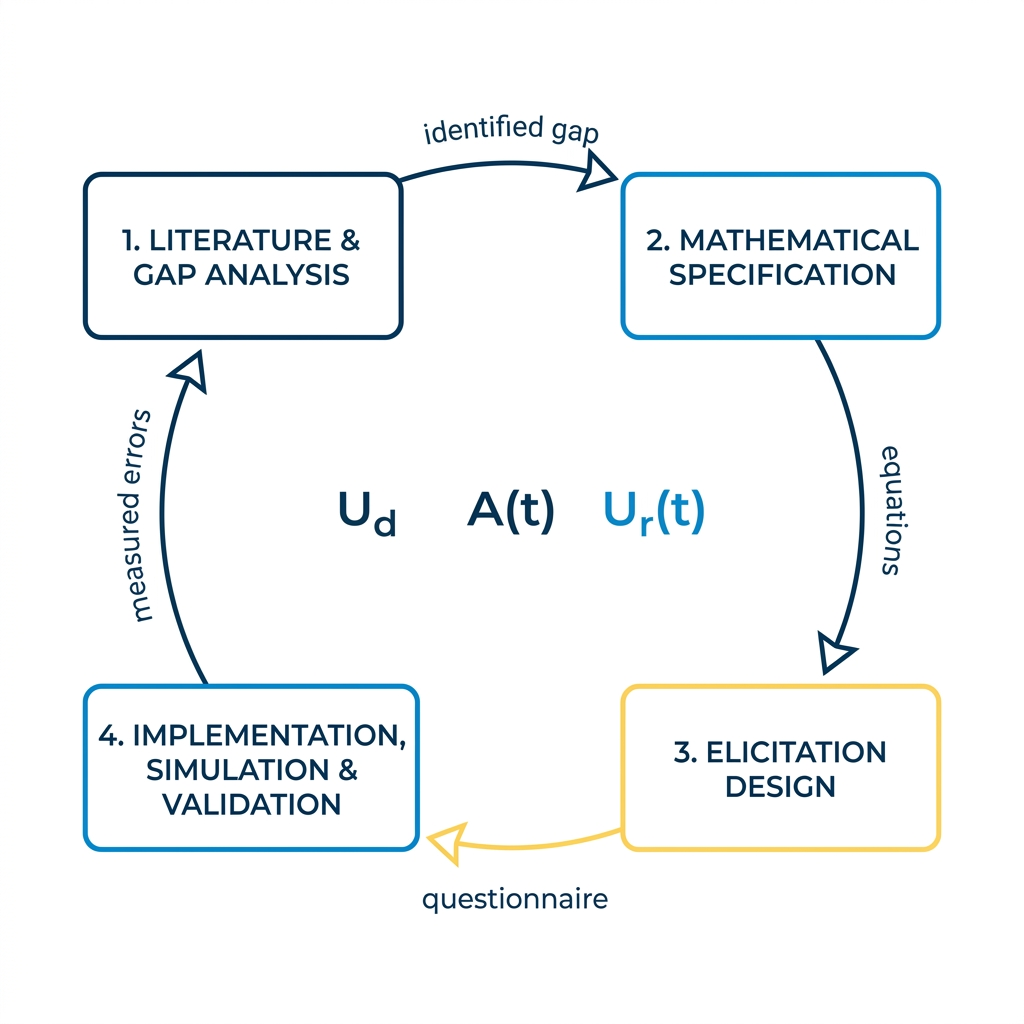
\includegraphics[width=0.85\linewidth]{Images/4.Operations/test_learn_loop.png}
    \caption{The agile Test-and-Learn iteration loop of the R\&D operation.}
    \label{fig:todraw_loop}
\end{figure}

%% ═══════════════════════════════════════════════════════════════════════════
\subsection{Mathematical Model}
\label{sec:math_framework}
%% ═══════════════════════════════════════════════════════════════════════════

This section states the model on its own terms: what real urgency and declared urgency are, how each is propagated across the network, and how their mismatch is scored. It intentionally leaves out tooling and interface choices, elicitation mechanics, and operational cadence, which are application decisions addressed separately in Section~\ref{sec:application}.

\subsubsection{Core Model: Real and Declared Local Urgency, and Network Propagation}

\paragraph{Local Real Urgency ($U_{r,\text{local}}$).}
Real urgency is not read from a single deadline-proximity signal; it is aggregated at each node from six independent KPI blocks, $\{\text{time}, \text{cap}, \text{perf}, \text{risk}, \text{cost}, \text{co2}\}$, each producing a partial urgency $u_m \in [0,1]$ or \texttt{None} when the underlying KPI data is unavailable. The aggregation is a weighted probabilistic OR, so that a single saturated block is sufficient to drive the local urgency toward its maximum, regardless of how well the other blocks score:
\begin{equation}
    U_{r,\text{local}} = 1 - \prod_{m} (1 - u_m)^{\omega_m},
    \label{eq:ur_local}
\end{equation}
where $\omega_m \ge 0$ is the aggregation weight of block $m$, and the product runs over blocks with available data. Table~\ref{tab:ur_blocks} gives, for each block, its schematic formula and what it measures; the notation $[x]_+ = \max(x, 0)$ denotes the positive part, and the per-term weights ($\alpha_i$, $\beta_i$) are renormalised over the terms whose data is actually available.

\begin{table}[H]
\centering
\caption{The six real urgency blocks: formula and explanation.}
\label{tab:ur_blocks}
\small
\begin{tabularx}{\linewidth}{l >{\raggedright\arraybackslash}p{4.6cm} X}
\toprule
\textbf{Block} & \textbf{Formula} & \textbf{Explanation} \\
\midrule
$u_{\text{time}}$ & $P(L > d^\ast - t) + \kappa_{\text{retard}}[r]_+ - \kappa_{\text{avance}}[-r]_+$ & Probability that the lead time $L$, modelled as Normal($\mu$, $\sigma$), exceeds the time left before the next active deadline $d^\ast$; forced to $1$ once the deadline is passed. The planning term $r$ compares theoretical progress with reported progress: a milestone behind plan raises the block, one ahead of plan lowers it. \\
\midrule
$u_{\text{cap}}$ & $\alpha_1\bigl(1-\tfrac{V_{\text{rem}}}{V_{\max}}\bigr) + \alpha_2\bigl(1-\tfrac{W_{\text{rem}}}{W_{\max}}\bigr) + \alpha_3\bigl[\tfrac{D-\Phi}{D}\bigr]_+$ & Saturation of the node's capacity: how little storage volume and weight remain, plus the fraction of demand $D$ not covered by the current flow rate $\Phi$. \\
\midrule
$u_{\text{perf}}$ & $1 - \text{OEE}$ & Complement of Overall Equipment Effectiveness (availability $\times$ performance $\times$ quality): the lower the productive health of the critical resource, the higher the urgency. \\
\midrule
$u_{\text{risk}}$ & $1-\exp\bigl(-p_{\text{fail}} \times t_{\text{recov}} \times \text{sev}/T_{\text{ref}}\bigr)$ & Expected unavailability: failure probability times recovery time times impact severity, normalised by a reference horizon $T_{\text{ref}}$, then combined by probabilistic OR with the environmental and political exposure terms. \\
\midrule
$u_{\text{cost}}$ & $\beta_1\,\tfrac{c_{\text{op}}-c_{\text{nom}}}{c_{\text{nom}}} + \beta_2\,[\text{tariff}-1]_+ + \beta_3\,\tfrac{c_{\text{stock}}}{C_{\text{ref}}}$ & Financial stress: drift of operating cost above its nominal value, tariff multiplier above neutral, and storage cost relative to a reference cost. \\
\midrule
$u_{\text{co2}}$ & $\bigl[\tfrac{e - e_{\text{target}}}{e_{\max}-e_{\text{target}}}\bigr]_+$ & Normalised overshoot of measured emissions $e$ above the target, saturating at the maximum threshold. \\
\bottomrule
\end{tabularx}
\end{table}

% -----------------------------------------------------------------------------
% REMARQUE MÉTHODOLOGIQUE DÉTAILLÉE : FONCTIONS DE TRANSFERT ET NORMALISATION ADIMENSIONNELLE
% -----------------------------------------------------------------------------
% Pour répondre à la question du jury/examinateur ("Comment comparer des jours, des € et des % sans soustraire des pommes et du tissu ?") :
% 1. Chaque KPI physique brut (avec dimension : jours, €, kg, %) passe par une fonction de transfert u_m(·).
% 2. u_m(·) est une application mesurable de R_physique -> [0, 1] adimensionnel :
%    - u_m = 0.0 : état nominal / sérénité opérationnelle (aucun risque).
%    - u_m = 1.0 : saturation du bloc / rupture imminente ou consommée.
% 3. C'est ce rebasage adimensionnel strict sur [0, 1] qui rend légitime l'agrégation par Noisy-OR (Eq. 1)
%    et la confrontation asymétrique avec l'urgence déclarée U_d (élicitée par AHP sur [0, 1])
%    dans l'équation d'adéquation A(t) = 100 * (1 - Pénalité(U_d - U_r)).
% -----------------------------------------------------------------------------

Two conventions make this aggregation unambiguous, since a bare formula does not by itself say what its bounds mean. First, each $u_m$ is engineered to carry the same meaning regardless of which raw KPI feeds it: $u_m \to 0$ means the block is healthy and contributes no urgency, $u_m \to 1$ means the block is saturated, that is, it has reached the point past which it cannot make the node any more urgent, whether that point is a missed deadline, a fully depleted buffer, or a near-certain failure. This use of ``saturated'' is a design choice made for this model, not a term imported as-is from the literature; it is what makes the noisy-OR product in Equation~\ref{eq:ur_local} valid across six structurally different blocks, since the product only requires each factor to share the same $[0,1]$ urgency scale, not the same physical units or the same statistical behaviour between $0$ and $1$. Second, a block whose data is \texttt{None} is excluded from the product entirely rather than assigned a value: because the product runs only over blocks with available data, a missing block neither raises nor lowers $U_{r,\text{local}}$, it is simply absent from the evidence, and the remaining weights are renormalised over what is left. Treating the six blocks as comparable on $[0,1]$ is therefore a modelling commitment, not a measured property, and Section~\ref{sec:limitations} lists it among the framework's stated limitations.

Two lifecycle status rules are applied before aggregation: a node marked \texttt{DONE} has its effective local $U_r$ forced to $0.0$ (a completed task carries no further physical risk), while a node marked \texttt{ABANDONED} has it forced to $1.0$ (complete failure). These rules are applied identically whether the local urgency comes from the analytic blocks above or from the Monte Carlo estimate of the time block described below.

\paragraph{Why These Six Blocks: A Rupture-Risk-Driven Selection.}
The six blocks were not chosen as an arbitrary KPI shortlist. The selection started from the question that defines urgency in a supply chain: \emph{what mechanisms make the risk of a delivery rupture rise?} A rupture, that is the inability to deliver at the agreed time, place, quantity, and quality, is the terminal event the urgency signal must anticipate~\autocite{heckmann2015critical}. Working backwards from that event, and consistently with indicator-based supply risk monitoring~\autocite{mokhtar2019supplier}, four \emph{direct causal mechanisms} and two \emph{arbitration variables} were identified:

\begin{itemize}
    \item \textbf{Time erosion ($u_{\text{time}}$)}: the remaining slack between deadline and realistic lead time. Time is the only non-compressible resource: whatever the state of the other indicators, a task whose slack reaches zero can no longer be saved, which makes deadline proximity the variable most directly tied to operational urgency~\autocite{cohen2021assigning,bojarski2021,sun2020combating,sawik2013integrated}.
    \item \textbf{System saturation ($u_{\text{cap}}$)}: queues, transport capacity, workshop load, and bottlenecks. A saturated system introduces hidden waiting delays on top of the nominal lead time, so capacity stress raises non-delivery risk even when the announced lead time looks safe~\autocite{tomlin2006value,hosseini2019resilient,taghavi2024sustainable}.
    \item \textbf{Critical-resource performance ($u_{\text{perf}}$)}: drift in the performance of the resource that produces the part. OEE is used as a composite proxy (availability $\times$ performance $\times$ quality) rather than a single machine metric, because precise performance data is rarely accessible on the supplier side~\autocite{mokhtar2019supplier,hlioui2017joint}.
    \item \textbf{Adverse-event exposure ($u_{\text{risk}}$)}: the expectation of unavailability caused by a disruption, computed as failure probability $\times$ recovery time $\times$ impact severity, composed with environmental and political exposure. The default incident probability (0.02) is revised weekly from declared events through the Bayesian operator of Section~\ref{sec:weekly_cycle} over a $n_0 = 26$ iteration window; this block builds on the DIN supplier risk scorer~\autocite{kabouche2025scoring} and on probabilistic ripple-effect models~\autocite{hosseini2020ripple,liu2021robust,hosseini2020bayesian}.
    \item \textbf{Financial flexibility ($u_{\text{cost}}$)}: expediting surcharges, tariff rises, storage costs. Cost drift is not a rupture cause in itself but a stress indicator of the chain (paying premium express transport to avoid a physical rupture is a measurable symptom that the system is straining), and it bounds which corrective actions remain economically viable~\autocite{shen2019managing,tomlin2006value}.
    \item \textbf{Carbon overshoot ($u_{\text{co2}}$)}: emissions above target. Like cost, it is an arbitration criterion rather than a rupture mechanism: it only becomes decisive when the regulatory or ESG constraint genuinely restricts the set of admissible responses, typically the ship-vs-air trade-off~\autocite{hoen2014effect,smartfreight2023glec,iso14083}.
\end{itemize}

Each candidate indicator was screened against four filter questions, summarised in Table~\ref{tab:block_selection}: only indicators passing all four were retained, which yields a set of four direct causes plus two arbitration variables and explains why the list is six blocks rather than four or eight.

\begin{table}[H]
\centering
\caption{Selection filter applied to each candidate KPI block.}
\label{tab:block_selection}
\small
\begin{tabularx}{\linewidth}{lX}
\toprule
\textbf{Criterion} & \textbf{Question asked of each candidate indicator} \\
\midrule
Causal link & Does the indicator have a plausible mechanism linking it to delivery rupture? \\
\midrule
Observability & Can it be measured or credibly estimated from client, supplier, or planning data? \\
\midrule
Actionability & Can an operator act on it, or use it to decide? \\
\midrule
Non-redundancy & Does it add information not already carried by a retained indicator? \\
\bottomrule
\end{tabularx}
\end{table}

At this stage the selection remains a \emph{conceptual} construction: it must still be confirmed by the real availability of the underlying data and by sensitivity tests verifying that each block contributes useful information to the aggregate (Section~\ref{sec:limitations}).

\begin{figure}[H]
    \centering
    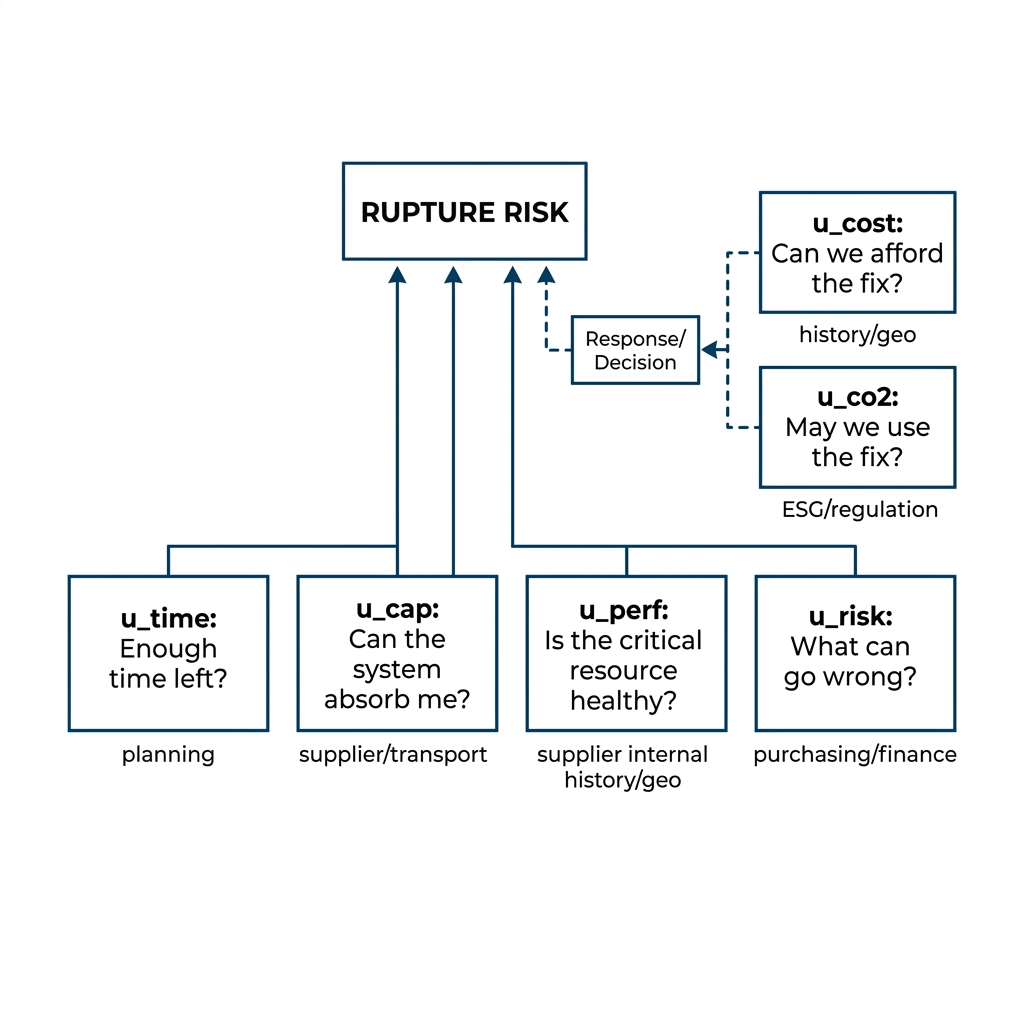
\includegraphics[width=0.85\linewidth]{Images/4.Operations/causal_tree_blocks.png}
    \caption{Causal structure behind the six-block selection: four direct rupture mechanisms and two arbitration variables.}
    \label{fig:todraw_blocks}
\end{figure}

\paragraph{Local Declared Urgency ($U_{d,\text{local}}$).}
Symmetrically to real urgency, declared urgency is not read as a single free-text estimate: it is reconstructed from a structured elicitation, so that it can be scored, propagated, and compared to $U_{r,\text{local}}$ on the same $[0,1]$ scale. At each node, the operator compares four criteria pairwise through the Analytic Hierarchy Process (\gls{ahp}), which yields a consistency-checked weight $w_j$ per criterion, then rates each criterion on a severity scale $s_j \in \{1, \ldots, 9\}$. Local declared urgency is the weight-averaged severity, rescaled to $[0,1]$:
\begin{equation}
    U_{d,\text{local}} = \sum_{j=1}^{4} w_j\,\frac{s_j - 1}{8}, \qquad \sum_{j=1}^{4} w_j = 1.
    \label{eq:ud_local}
\end{equation}
The elicitation tool itself, its four criteria, and the consistency gate that rejects an incoherent weight vector before it reaches this formula are application choices, described in Section~\ref{sec:ahp_tool}. What matters at this stage is that $U_{d,\text{local}}$ and $U_{r,\text{local}}$ (Equation~\ref{eq:ur_local}) are both bounded, node-local quantities in $[0,1]$ before either one is propagated, since the propagation equations below require both of them already defined.

\paragraph{Network Propagation.}
Declared urgency $U_d$ propagates \emph{downstream}, from the final customer (rank~0) toward raw-material suppliers, while real urgency $U_r$ propagates \emph{upstream}, from suppliers toward the final customer, using a leaky product rule that keeps both signals bounded in $[0,1]$ and monotonically increasing as more neighbours become urgent:
\begin{align}
    U_{d,i} &= 1 - \bigl(1 - U_{d,\text{local},i}\bigr) \prod_{k \in \text{Succ}(i)} \bigl(1 - \gamma_{ik} U_{d,k}\bigr), \label{eq:ud_prop} \\
    U_{r,i} &= 1 - \bigl(1 - U_{r,\text{local},i}\bigr) \prod_{j \in \text{Pred}(i)} \bigl(1 - \beta_{ji} U_{r,j}\bigr), \label{eq:ur_prop}
\end{align}
where $\gamma_{ik} \in [0,1]$ is the downstream attenuation coefficient on arc $(i,k)$ and $\beta_{ji} \in [0,1]$ is the upstream amplification coefficient on arc $(j,i)$. Backup arcs are purely documentary and inert with respect to both propagations. Table~\ref{tab:propagation_components} details the propagation variables.

\begin{table}[H]
\centering
\caption{Component definitions for the network propagation equations.}
\label{tab:propagation_components}
\small
\begin{tabularx}{\linewidth}{llX}
\toprule
\textbf{Component} & \textbf{Type} & \textbf{Description} \\
\midrule
$U_{d,i}$, $U_{r,i}$ & Dependent variables & Propagated declared/real urgency at node $i$ \\
$U_{d,\text{local},i}$, $U_{r,\text{local},i}$ & Input variables & Local urgency at node $i$ after status-rule adjustment \\
$\gamma_{ik}$ & System parameter & Downstream (demand) attenuation coefficient on arc $i \to k$ \\
$\beta_{ji}$ & System parameter & Upstream (risk) amplification coefficient on arc $j \to i$ \\
$\text{Succ}(i)$, $\text{Pred}(i)$ & Structural sets & Nominal (non-backup) successors and predecessors of node $i$ \\
\bottomrule
\end{tabularx}
\end{table}

Propagation is recomputed incrementally: only the nodes downstream or upstream of a change (a submitted questionnaire, a revised KPI, a structural edit) are recalculated, rather than the full graph, which keeps the digital twin responsive as the network grows. Computation and propagation are triggered per node, not on a single synchronised clock: whenever a node's local urgency changes, whether from a submitted weekly review or a manual KPI edit, the system recomputes that node's aggregation and propagates the change through its upstream or downstream cone only (Section~\ref{sec:architecture}). Because each node is reviewed on its own weekly cadence rather than all at once, propagation across the network is continuous and asynchronous in practice, not a single global weekly batch; Section~\ref{sec:weekly_cycle} describes the review cadence itself.

\begin{figure}[H]
    \centering
    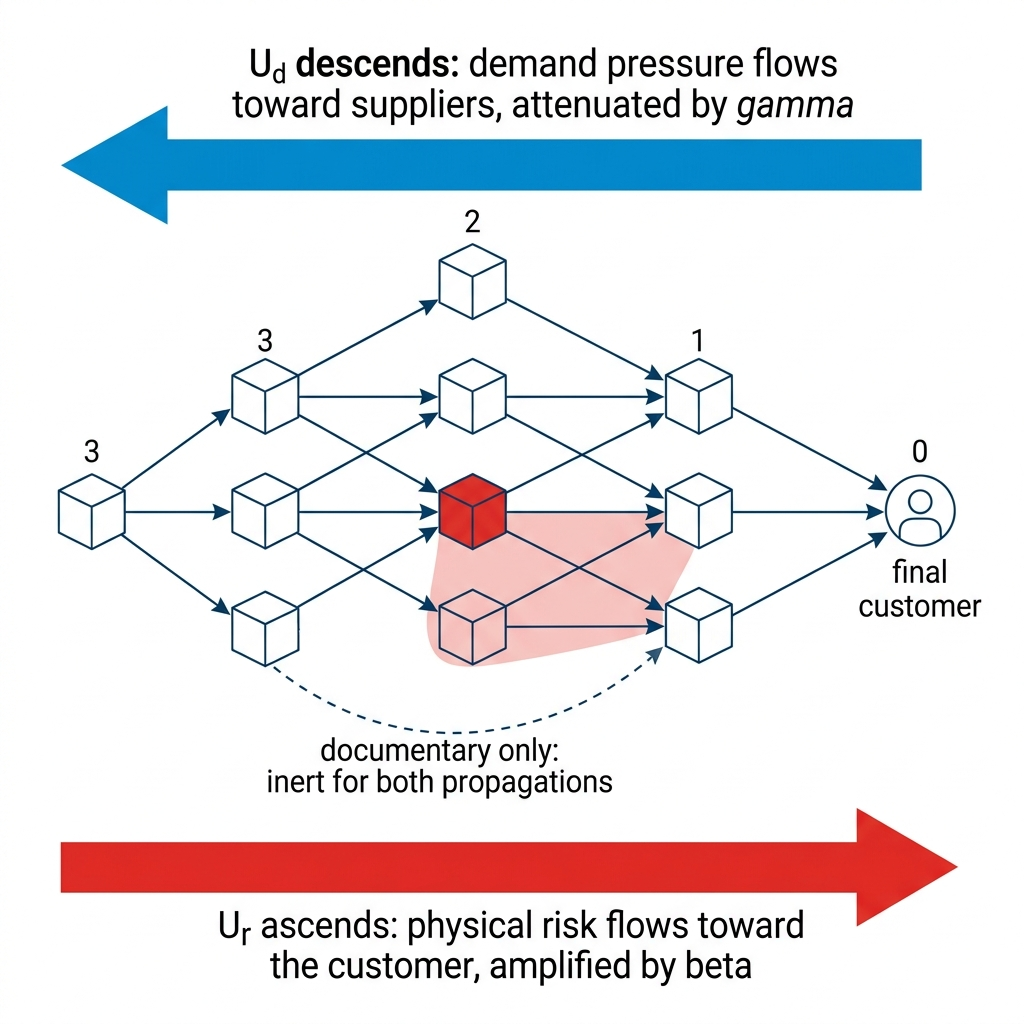
\includegraphics[width=0.85\linewidth]{Images/4.Operations/urgency_propagation.png}
    \caption{Bidirectional urgency propagation on the supply chain DAG.}
    \label{fig:todraw_propagation}
\end{figure}

\subsubsection{Core Model: Asymmetric Cognitive Adequacy (Prospect Theory)}

The mismatch between declared and real urgency is split into two named pathologies, false urgency $F$ (over-declaration, panic) and hidden risk $H$ (under-declaration, silent danger):
\begin{equation}
    F = \max(U_d - U_r,\, 0), \qquad H = \max(U_r - U_d,\, 0).
    \label{eq:fh}
\end{equation}
Drawing on Kahneman and Tversky's Prospect Theory~\autocite{kahneman1979prospect}, the two pathologies are penalised asymmetrically and with diminishing marginal sensitivity to large errors:
\begin{equation}
    \text{penalty} = \lambda_{\text{under}} H^{\alpha} + \lambda_{\text{over}} F^{\alpha},
    \label{eq:penalty}
\end{equation}
and the penalty is rescaled into an adequacy score $A \in [0, 100]$ through an exponential mapping bounded by the penalty of a maximal one-sided error:
\begin{equation}
    A = 100 \times \frac{\exp(-\text{penalty}) - \exp(-\text{penalty}_{\max})}{1 - \exp(-\text{penalty}_{\max})}, \qquad \text{penalty}_{\max} = \max(\lambda_{\text{under}}, \lambda_{\text{over}}).
    \label{eq:At}
\end{equation}
Table~\ref{tab:adequation_components} lists the parameters, with their governing constraint $\lambda_{\text{under}} > \lambda_{\text{over}}$: a coordinator who panics wastes premium transport capacity, but a coordinator who under-reports risk misses the window to prevent a line stoppage, so under-declaration is priced more expensively.

\begin{table}[H]
\centering
\caption{Component and parameter definitions for the asymmetric adequacy equations.}
\label{tab:adequation_components}
\small
\begin{tabularx}{\linewidth}{llXl}
\toprule
\textbf{Component} & \textbf{Type} & \textbf{Description} & \textbf{Default} \\
\midrule
$F$ & Dependent variable & False urgency (over-declaration) & n/a \\
$H$ & Dependent variable & Hidden risk (under-declaration) & n/a \\
$\lambda_{\text{under}}$ & System parameter & Penalty weight on hidden risk & $2.25$ \\
$\lambda_{\text{over}}$ & System parameter & Penalty weight on false urgency & $1.0$ \\
$\alpha$ & System parameter & Psychophysical curvature (diminishing sensitivity) & $0.88$ \\
$A$ & Dependent variable & Adequacy score, $100$ = perfect alignment & $[0,100]$ \\
\bottomrule
\end{tabularx}
\end{table}

The default $\lambda_{\text{under}}/\lambda_{\text{over}} = 2.25$ ratio reprises the loss-aversion coefficient measured by Kahneman and Tversky~\autocite{kahneman1979prospect,kahneman2011thinking}, and $\alpha = 0.88$ reprises their measured curvature of the value function. These defaults carry the status of literature-derived starting points, not measured properties of supply chain coordinators: they have not yet been validated empirically in this context, and their recalibration is one purpose of the validation campaign of Section~\ref{sec:serious_game}. Both the aggregation weights $\omega_m$ and the penalty parameters $(\lambda_{\text{under}}, \lambda_{\text{over}}, \alpha)$ are configurable per project rather than hard-coded, so that this recalibration requires no code change.

\subsubsection{Monte Carlo Estimate of the Time Block}
\label{sec:mc_criticality}

The analytic $u_{\text{time}}$ block assumes a Normal lead time at a single node. On a multi-tier network this assumption breaks: a node can only start when \emph{all} its predecessors have delivered, and the maximum of several skewed lead times has no convenient closed form. The module \texttt{mc/lead\_time.py} therefore replaces the analytic estimate with a stochastic one when enabled.

The simulation works in three steps. First, each node draws its lead time $L_i$ from a configurable distribution (lognormal, normal clipped to zero, or triangular). Second, completion times propagate along the DAG in topological order: a node starts when its last predecessor finishes ($S_i = \max_{j\in\text{Pred}(i)} C_j$) and completes after its own lead time ($C_i = S_i + L_i$). Third, the delay probability of each node is estimated as the fraction of draws in which it misses its deadline, $u_{\text{time}} = P(C_i > d_i)$, over $N=10\,000$ draws by default. A memory guardrail caps the simulation at $N \times n \le 5\times 10^7$ across $n$ nodes.

The estimate feeds directly into Equation~\ref{eq:ur_local} through a dedicated override point, so the aggregation, status rules, and propagation machinery are reused unchanged.

\subsubsection{Network Criticality Index}
\label{sec:criticality}

The criticality service (\texttt{services/criticite.py}) answers one question systematically: which node, if it failed completely, would cause the most damage to final-customer delivery? For every active node in turn, the service forces the node's local real urgency to $1.0$, re-runs the ascending propagation, and measures two deltas: the rise of $U_r$ at the final-customer nodes ($\Delta U_{r,\text{final}}$) and the largest rise anywhere in the network ($\Delta U_{r,\max}$). Every shock is run twice, once on the standard pipeline and once on an $\varepsilon$-regularised twin that carries the same computation in log-survival, $\ell(p) = -\ln(1-p)$, with urgency values clipped to $1-\varepsilon$ so that a survival product is never exactly zero. Nodes are ranked by $\Delta U_{r,\text{final}}$ first, then by $\Delta \ell_{\text{final}}$, then by name. The reason for that second key is the saturation behaviour described below.

A small example makes the mechanics concrete. Take a three-node chain, raw-material supplier $\to$ sub-assembly $\to$ final assembly, with upstream coefficients $\beta = 0.9$ then $0.7$, and a baseline where the sub-assembly node carries $U_{r} = 0.40$ and the final node $U_r = 0.28$. Forcing the sub-assembly node to $U_r = 1.0$ propagates to the final node as $1-(1-0.7\times1.0) = 0.70$, so its shock deltas are $\Delta U_{r,\text{final}} = 0.70-0.28 = 0.42$ and $\Delta U_{r,\max} = 1.0-0.40 = 0.60$ (Figure~\ref{fig:criticite}).

One behaviour of this index matters for interpretation: a node already saturated at $U_r \ge 1.0$ yields a delta of zero and sinks to the bottom of the ranking, since its risk is already realised in the baseline. In a network-wide crisis, where many nodes saturate at once, $\Delta U_r$ collapses to zero everywhere and the ranking degenerates, which is precisely the situation in which it would be most useful: nine of the nineteen turns of the campaign of Section~\ref{sec:serious_game} were saturated, and the exclusion rule used by hypothesis H3 was written for that reason.

The $\Delta \ell$ key is the answer to it. Because $\ell(p) = -\ln(1-p)$ is strictly increasing, $\Delta \ell_{\text{final}}$ and $\Delta U_{r,\text{final}}$ are two monotone transforms of the same shocked urgency at the final customer, so outside saturation they induce the same order and the ranking is unchanged; this is stated as a property-based invariant and tested as one. Inside saturation the clip that flattens $\Delta U_r$ does not flatten $\Delta \ell$, which keeps measuring how much deeper the shock drives an already saturated network, so the nodes that $\Delta U_r = 0$ made indistinguishable are separated again. Measured on the campaign turns, the number of turns on which the deep suppliers can be ordered at all rises from 10 to 17 out of 19.

\begin{figure}[H]
    \centering
    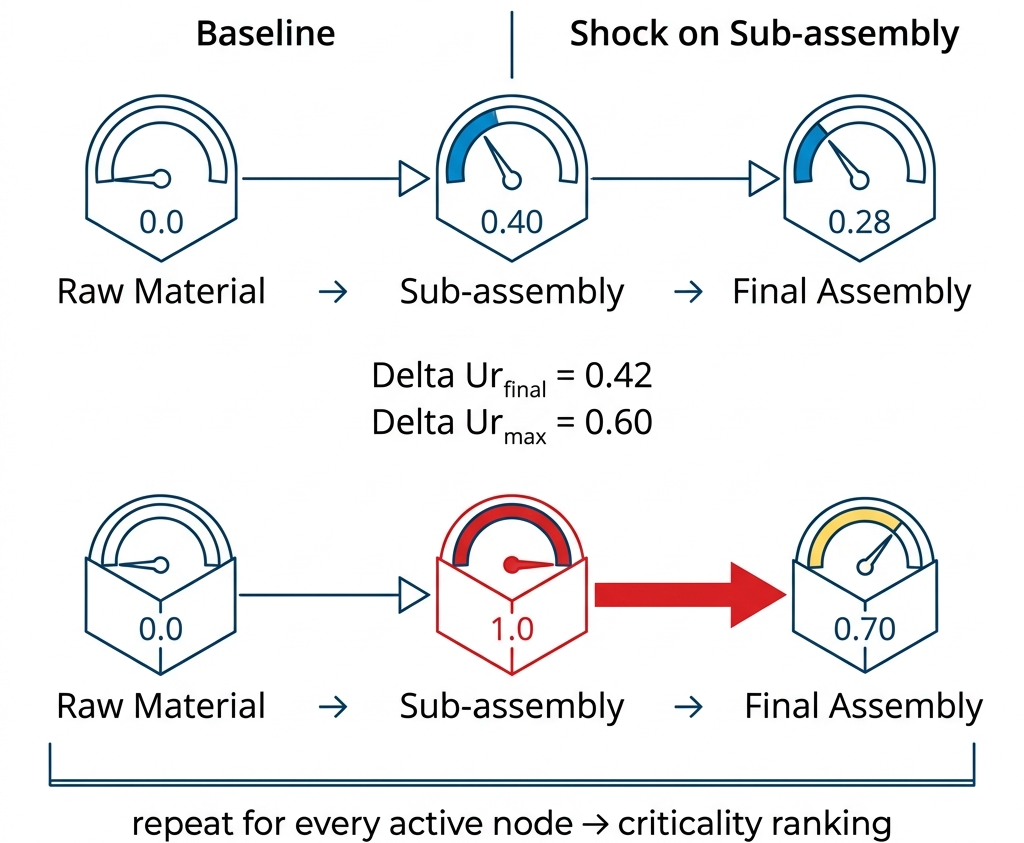
\includegraphics[width=0.85\linewidth]{Images/4.Operations/shock_simulation.png}
    \caption{One iteration of the systematic shock simulation behind the criticality index.}
    \label{fig:todraw_shock}
\end{figure}

\paragraph{Probabilistic Criticality.}
The sweep above answers what happens if a node fails \emph{completely}, which is a worst case rather than an expectation. A second entry point answers the distributional question on the same machinery. Instead of forcing $U_{r,\text{local}} = 1.0$, it draws shock severities from the graduated flat-rate severities of the calibrated event engine: minor, major and critical failures at $0.4$, $0.7$ and $1.0$, and financial alerts at $0.3$, $0.6$ and $0.9$, the two families weighted equally and, within a family, weighted by decreasing field frequency ($0.6$, $0.3$, $0.1$), since benign incidents are markedly more common than outright defaults. Each draw is applied as a ratchet, $\max(U_{r,\text{local}}, \text{severity})$, on the same principle as the event engine: a failure never improves a node's state. The whole batch is then propagated in one vectorised pass, in duplicate for $\Delta U_r$ and $\Delta \ell$. Each node receives $P(\Delta U_{r,\text{final}} > 0.2)$ and the median and ninth-decile of its $\Delta \ell_{\text{final}}$ distribution. The computation is read-only, seeded and deterministic, so the same inputs give the same ranking.

\begin{figure}[H]
    \centering
    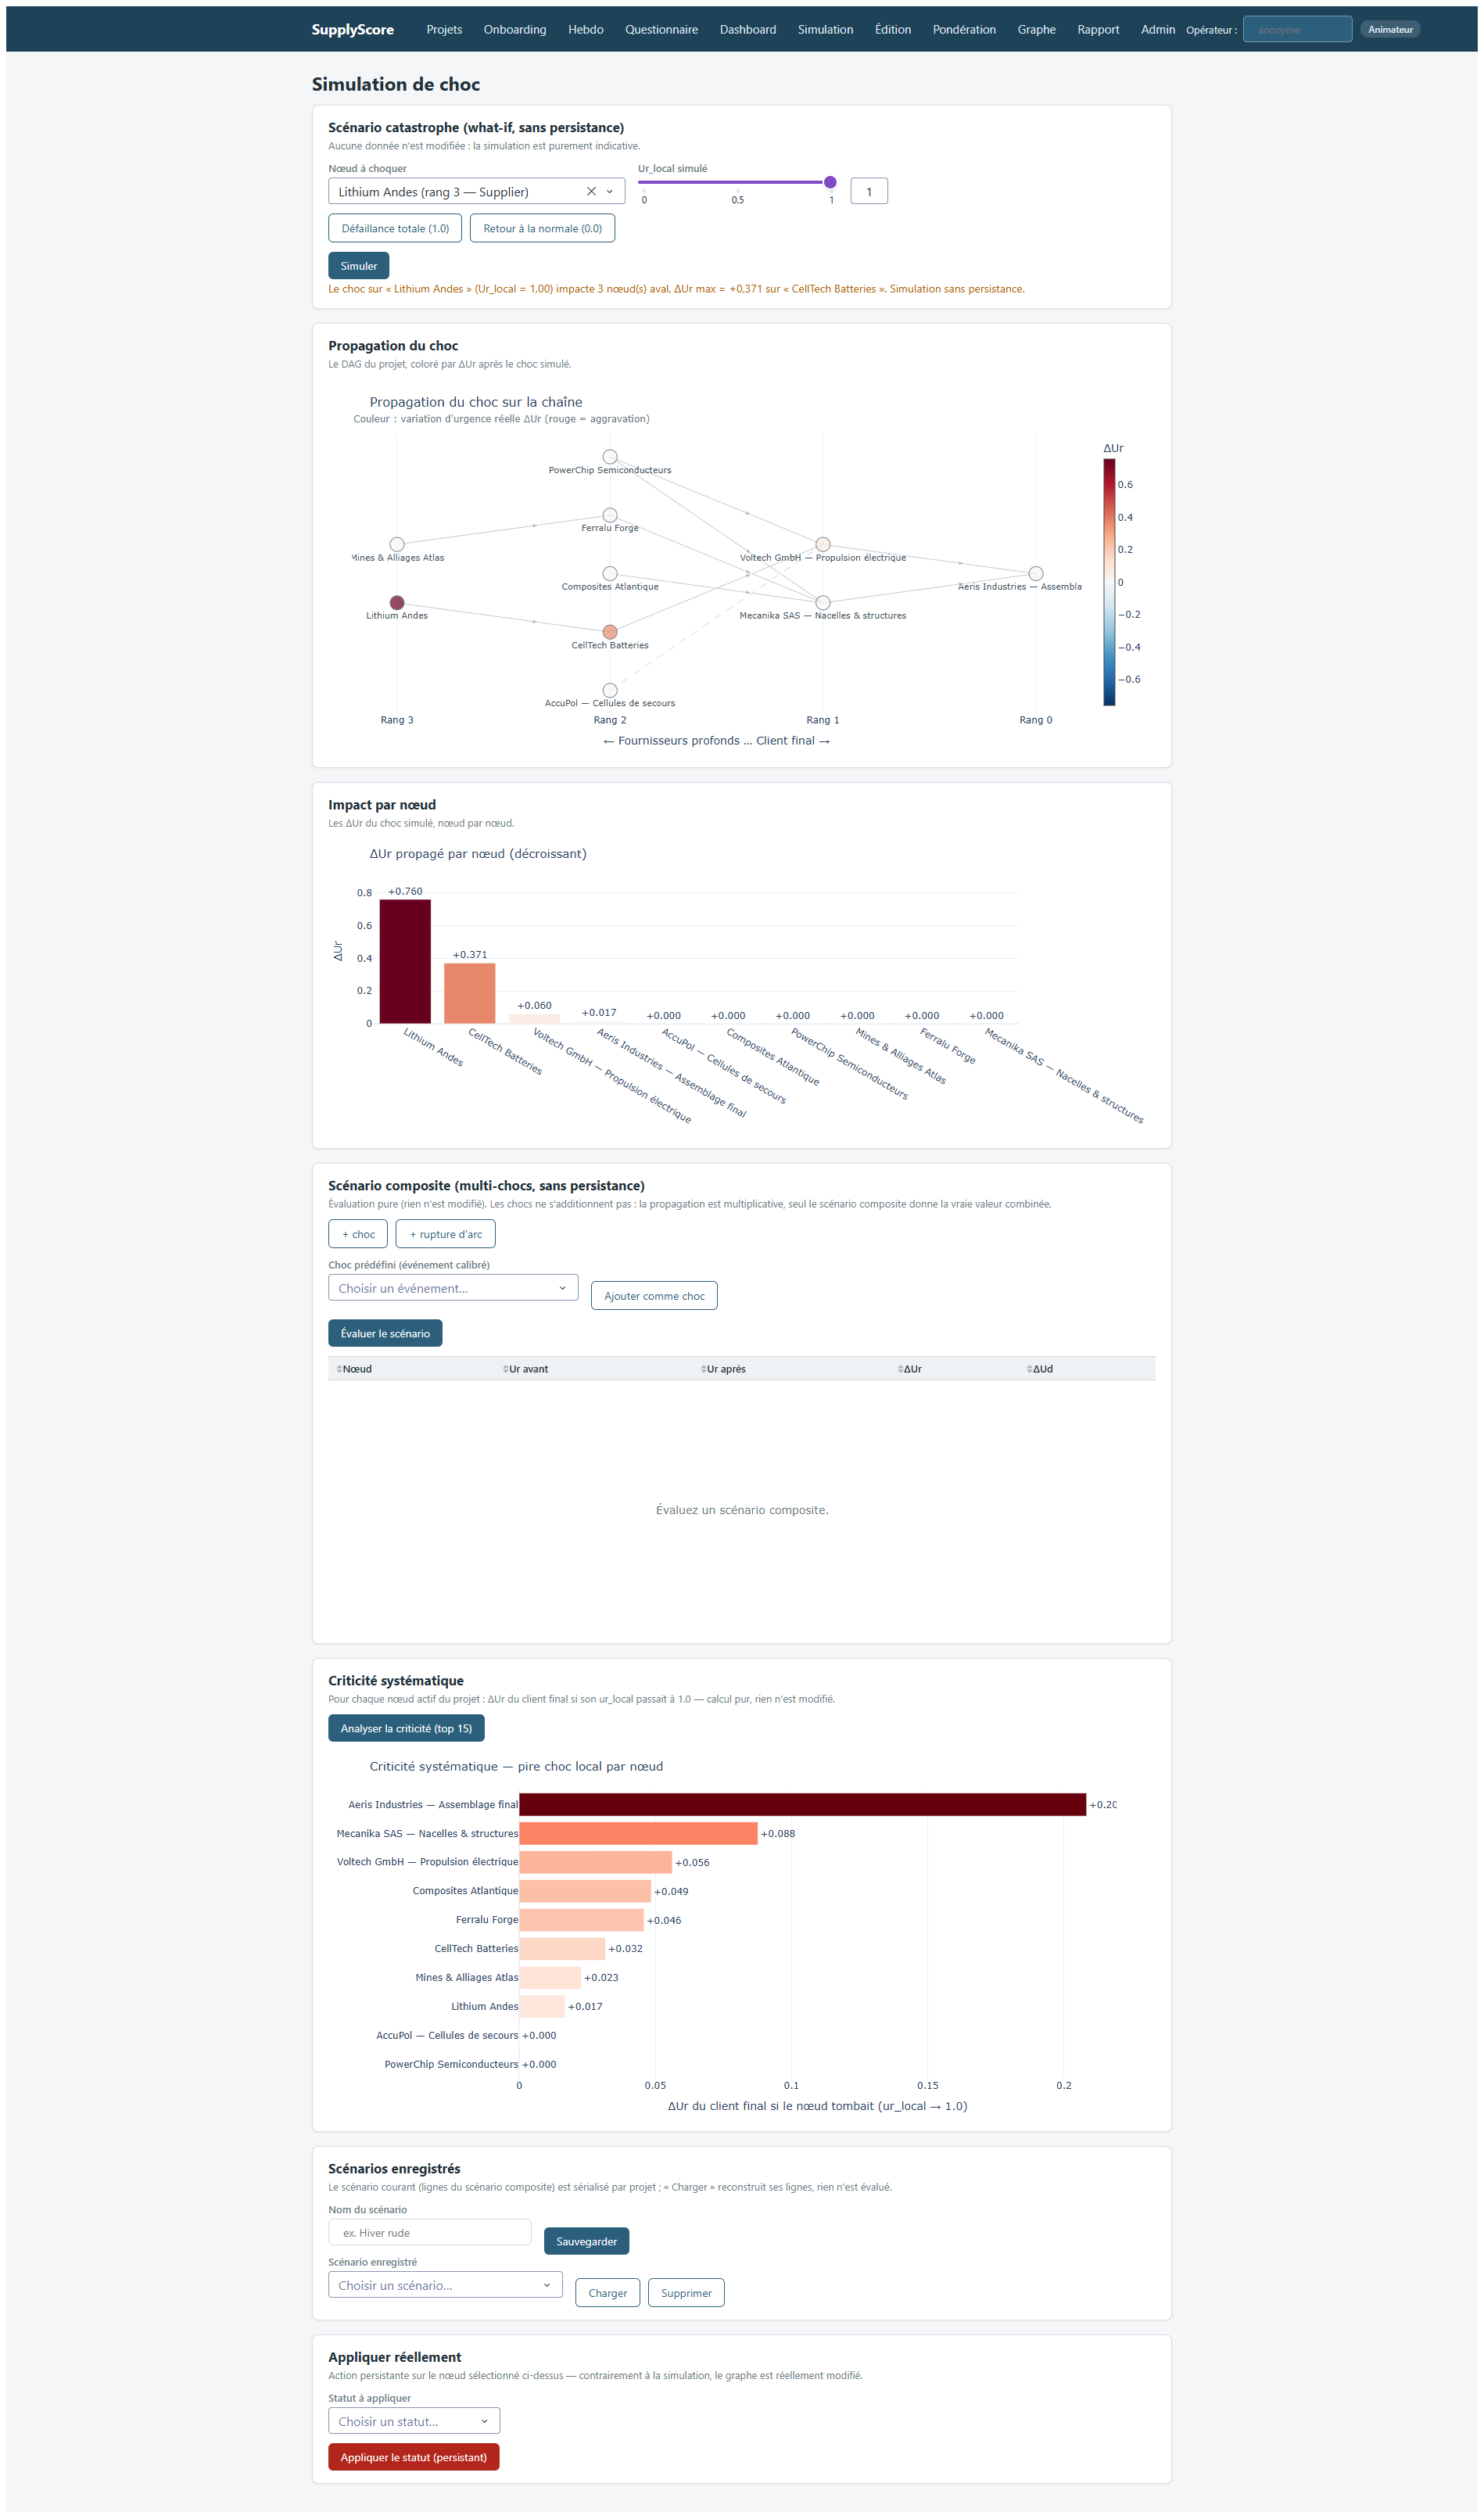
\includegraphics[width=0.85\linewidth]{Images/4.Operations/criticite.png}
    \caption{Network criticality ranking after a systematic shock simulation.}
    \label{fig:criticite}
\end{figure}

%% ═══════════════════════════════════════════════════════════════════════════
\subsection{Application and Implementation Choices}
\label{sec:application}
%% ═══════════════════════════════════════════════════════════════════════════

The model above is deliberately silent on tooling. This section describes how each mathematical object it defines is actually elicited from an operator, computed inside the running system, exposed back to a coordinator, and kept safe: the system architecture, the AHP and Fuzzy-BWM/PROMETHEE elicitation tools, the weekly operating cycle and event engine that keep KPI data current, and the explainability, export, and hardening capabilities built on top.

\subsubsection{System Architecture}
\label{sec:architecture}

Several design guarantees relied upon elsewhere in this document, auditability, multi-tenant isolation, deterministic testing, are architectural choices, not mathematical ones, and are described here on their own.

\paragraph{Single facade.} All operations go through one orchestrating facade
(\texttt{services/}\allowbreak\texttt{orchestrator.py}), which coordinates the mathematical core, the
graph repository, and the persistence layers behind a single thread-safe entry
point. The web interface, the command-line entry point, and the test suite all
drive the system exclusively through this facade; there is no second write path.

\paragraph{Multi-tenant persistence.} Data is split between one global registry
database (projects, nodes, arcs, milestones, scenarios, registry-level audit) and
one SQLite database per node holding its private operational history (KPI
snapshots, AHP assessments, weekly reviews, urgency history, declared events, and
a per-node audit log). This isolation prevents write contention between operators
reviewing different nodes and enforces the boundary that one supplier's raw
history is not readable through another supplier's records.

\paragraph{Gatekeeper writes.} Every business write crosses a single mutation
service that whitelists the touched fields, validates ranges, diffs against the
current state (a no-op write leaves no trace), records the change in the audit
log with its author and source, and synchronises the in-memory graph. Audit
tables are strictly immutable, including from the administration interface:
the "no silent data loss" guarantee is enforced here, not by convention.

\paragraph{Graph and propagation.} The network lives in an in-memory graph
repository (networkx-backed; a Neo4j adapter is scaffolded but out of scope).
Propagation is incremental: only the upstream/downstream cones of nodes whose
local urgency actually changed are recomputed, which keeps the twin responsive
at the 1000+-node scale validated by dedicated performance benchmarks.

\begin{figure}[H]
    \centering
    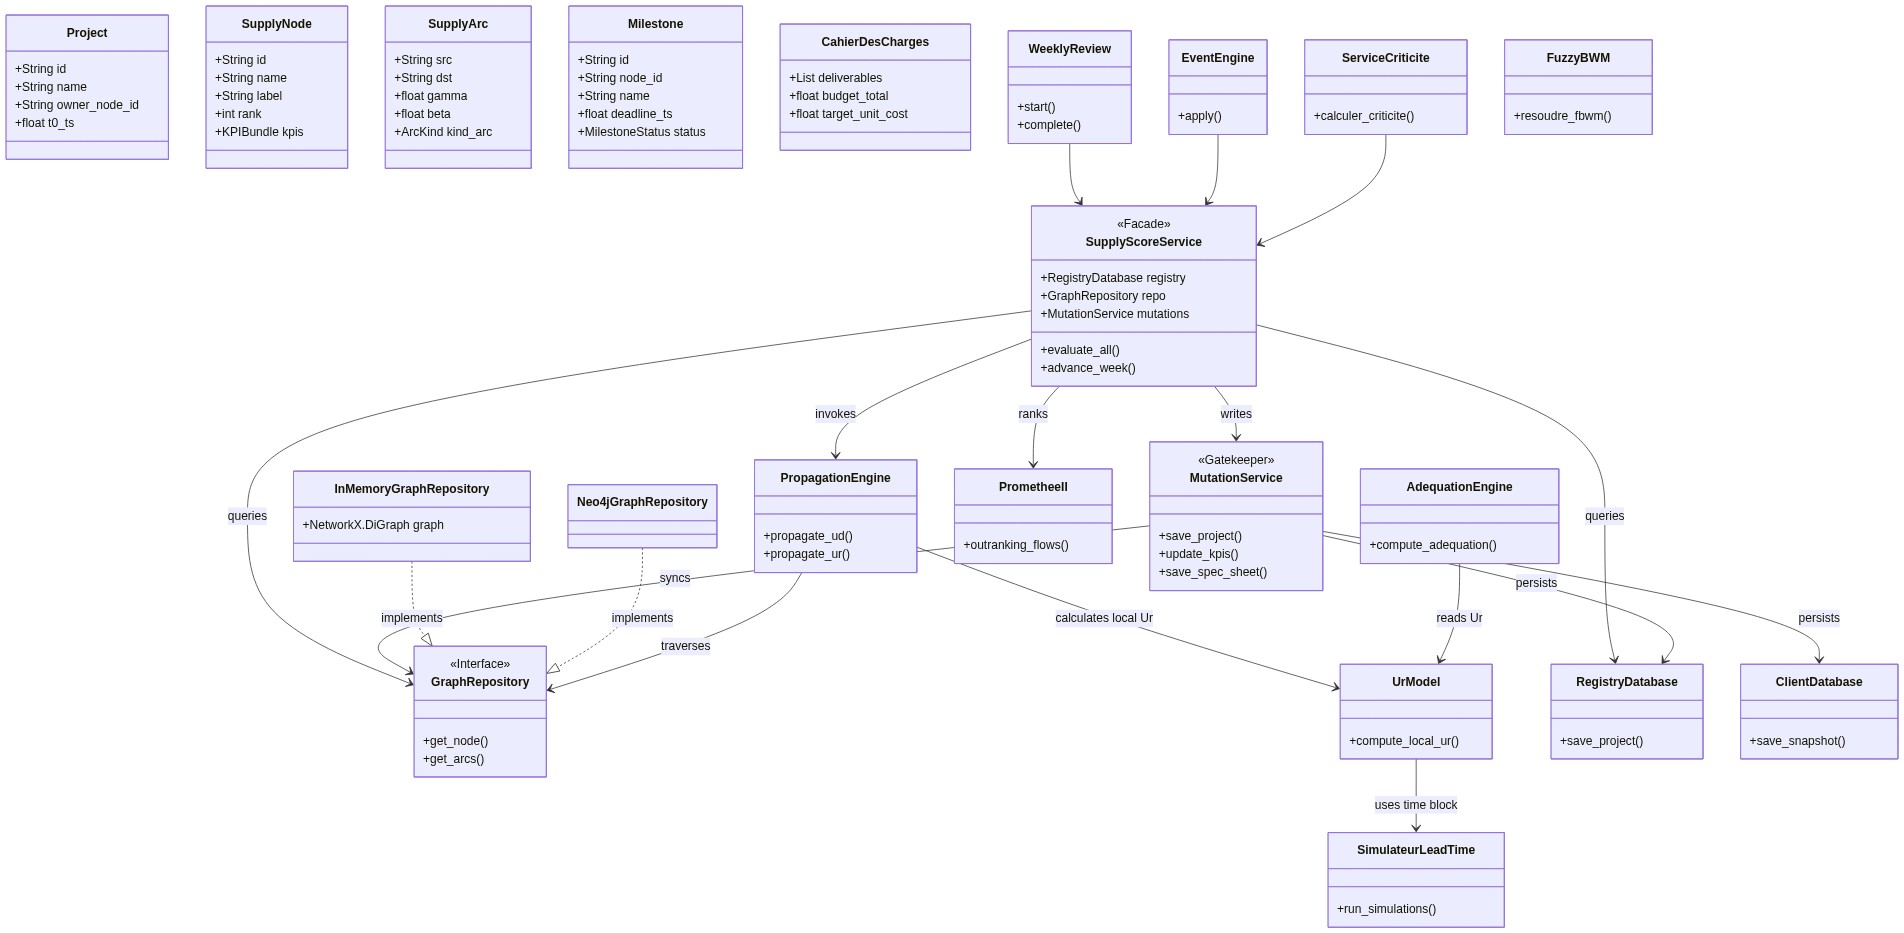
\includegraphics[width=0.85\linewidth]{Images/4.Operations/uml_architecture.png}
    \caption{Doxygen-generated UML view of the SupplyScore architecture: single facade, gated writes, multi-tenant persistence.}
    \label{fig:todraw_architecture}
\end{figure}

\paragraph{Decoupled clocks.} Each project carries its own clock: a system clock
for live use, a game clock advancing week by week for serious-game sessions, and
a fixed clock for deterministic tests. The weekly cycle, milestone pressure, and
event timestamps all read the project clock, never the wall clock directly,
which is what makes a compressed serious-game campaign (Section~\ref{sec:serious_game})
possible without touching the model.

\subsubsection{Expert Criteria Weighting: The AHP Elicitation Model}
\label{sec:ahp_tool}

The Python module \texttt{core/ahp.py} implements the Saaty
eigenvector method for a 4-criterion questionnaire administered through the weekly
review page, and is the tool that produces $U_{d,\text{local}}$ (Equation~\ref{eq:ud_local}). The four criteria are:

\begin{enumerate}[label=\textbf{C\arabic*.}]
    \item \textit{Operational impact}: ``If this task fails, what is the downstream
          consequence?''
    \item \textit{Time window}: ``How long before the situation becomes irredeemable?''
    \item \textit{Downstream dependencies}: ``How many tasks are blocked waiting for
          this one?''
    \item \textit{Recoverability}: ``Can we catch up if this task is late?''
          (inverted, where lower is worse)
\end{enumerate}

\paragraph{How the Four Criteria Were Chosen.}
The criteria set follows from two constraints, one cognitive and one structural. Cognitively, Saaty's method degrades as the number of pairwise-compared criteria grows: consistency becomes hard to maintain beyond roughly seven items, and each additional criterion adds $n-1$ comparisons to the operator's weekly workload~\autocite{saaty1990how,triantaphyllou2024}. Keeping $n=4$ limits the questionnaire to six comparisons, short enough for a weekly cadence. Structurally, the four questions mirror the way declared urgency is consumed downstream: C1 (impact) and C3 (dependencies) capture the \emph{severity} dimension that propagation amplifies across the network, C2 (time window) captures the \emph{slack} dimension confronted with the $u_{\text{time}}$ block of Section~\ref{sec:math_framework}, and C4 (recoverability) captures the \emph{resilience} dimension confronted with the recovery term of $u_{\text{risk}}$. Each declared criterion therefore has an operational counterpart in the computed signal, which is what makes the later $U_d$ vs.\ $U_r$ comparison meaningful rather than a comparison of unrelated quantities. Larger criteria sets (cost, sustainability) are deliberately routed to the F-BWM weighting of the KPI blocks instead (Section~\ref{sec:fbwm_promethee}), where the elicitation burden is lower.

\begin{figure}[H]
    \centering
    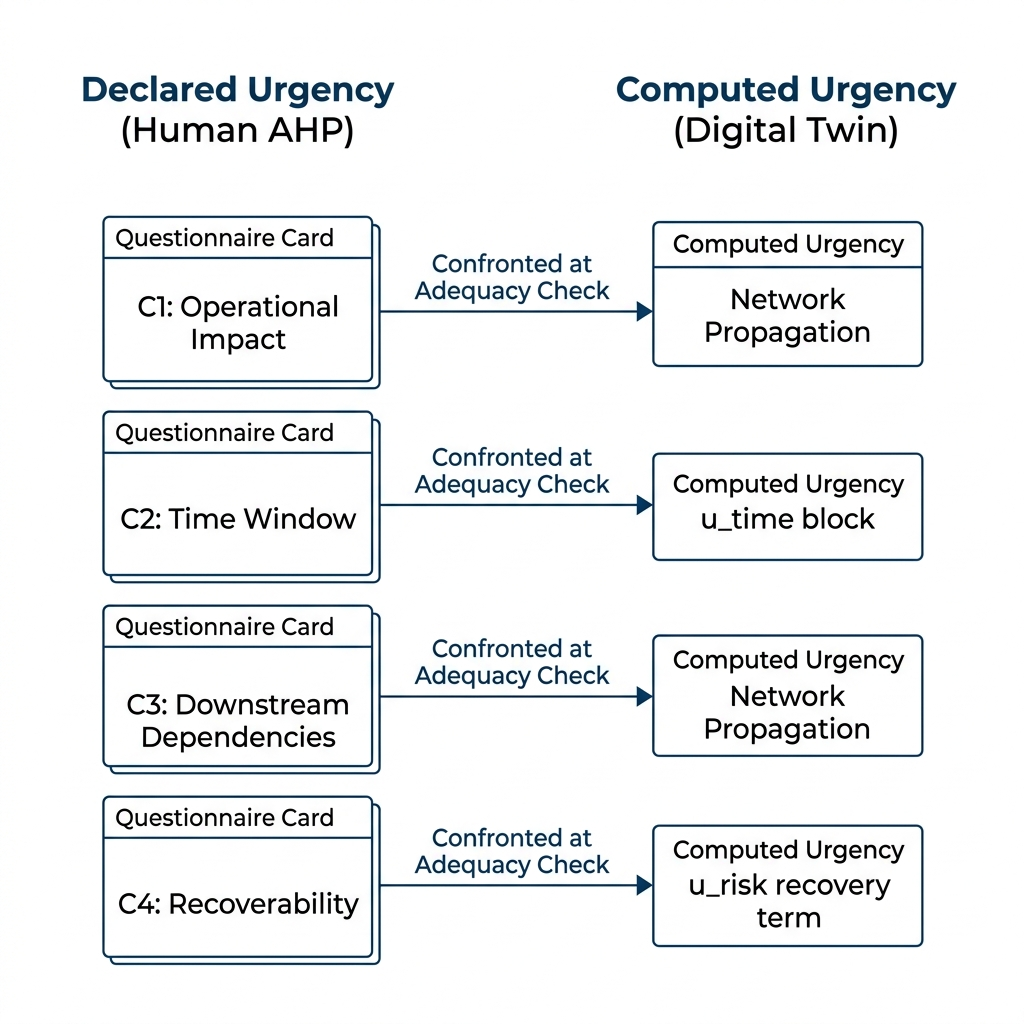
\includegraphics[width=0.85\linewidth]{Images/4.Operations/ahp_criteria_mapping.png}
    \caption{Correspondence between the four AHP criteria and their computed counterparts.}
    \label{fig:todraw_criteria}
\end{figure}

The consistency ratio is computed as:
\begin{equation}
    \gls{cr} = \frac{\gls{ci}}{\gls{ri}[n]},
    \label{eq:ahp_cr}
\end{equation}
where the components of the consistency assessment are defined in Table~\ref{tab:ahp_cr_components}.

\begin{table}[H]
\centering
\caption{Component definitions for the AHP consistency ratio equation.}
\label{tab:ahp_cr_components}
\small
\begin{tabularx}{\linewidth}{llX}
\toprule
\textbf{Component} & \textbf{Type} & \textbf{Description} \\
\midrule
$\gls{cr}$ & Dependent variable & Consistency Ratio of the pairwise comparison matrix \\
$\gls{ci}$ & Dynamic variable   & Consistency Index computed from the matrix principal eigenvalue \\
$\gls{ri}[n]$ & System parameter & Random Index for a matrix of size $n$ (from Saaty's reference table) \\
\bottomrule
\end{tabularx}
\end{table}

using Saaty's Random Index table. If $\gls{cr} > 0.10$, the interface flags the questionnaire as inconsistent and invites the operator to revise the most contradictory pairwise comparison before the assessment is accepted. Declared urgency is further smoothed with an exponential moving average ($\rho = 0.3$) across consecutive weekly assessments, absorbing transient stress spikes without erasing a sustained change in perception.

\begin{figure}[H]
    \centering
    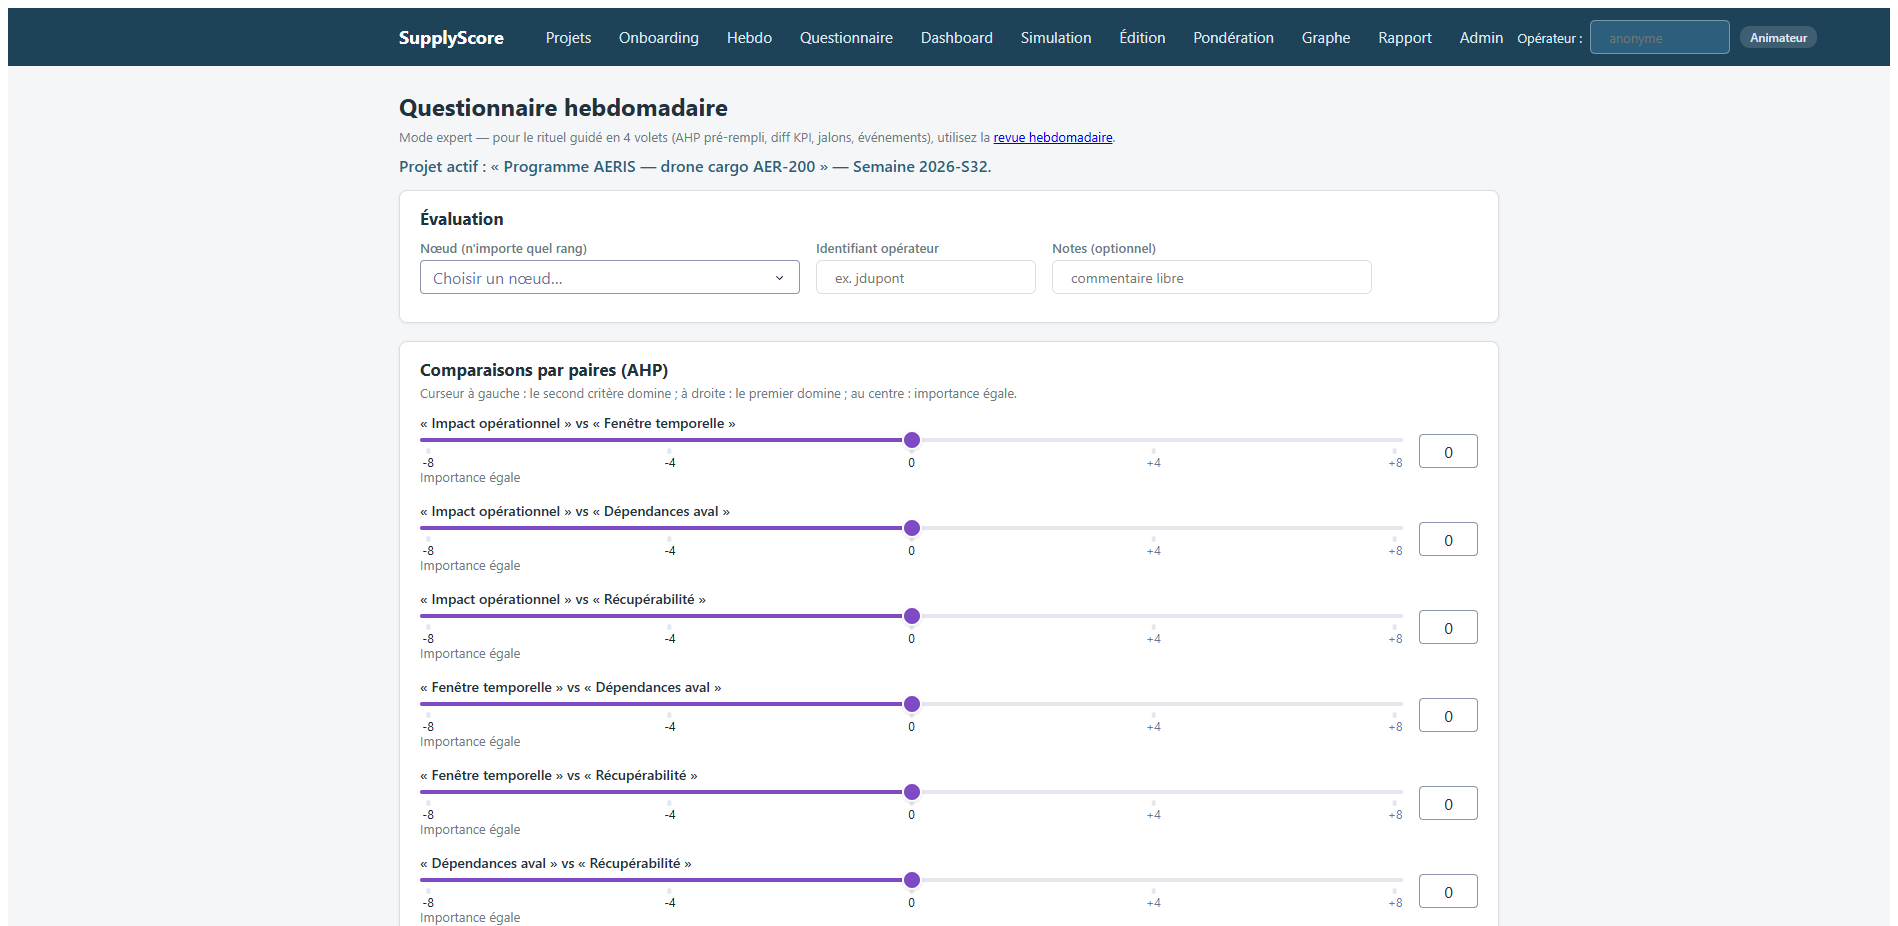
\includegraphics[width=0.85\linewidth]{Images/4.Operations/questionnaire_screenshot.png}
    \caption{AHP questionnaire page with the consistency-ratio validation gate.}
    \label{fig:todraw_questionnaire}
\end{figure}

AHP is viable for $U_d$ encoding in this context. The
$\gls{cr}$ validation gate, exercised by both worked examples and automated tests, detects and rejects cognitively inconsistent
expert inputs before they enter the network. Its behaviour with real operators is measured in the campaign of Section~\ref{sec:serious_game}.

%% ═══════════════════════════════════════════════════════════════════════════
\subsubsection{Stochastic Judgment Modeling: Fuzzy BWM and PROMETHEE II Network Outranking}
\label{sec:fbwm_promethee}
%% ═══════════════════════════════════════════════════════════════════════════

The modules \texttt{mcda/fbwm.py} and \texttt{mcda/promethee.py} implement
two complementary methods: F-BWM offers a lower-effort elicitation route than crisp AHP for
weighting the six KPI blocks, and PROMETHEE~II turns those weights into a network-wide,
non-compensatory ranking of nodes that complements the per-node adequacy score.

\paragraph{F-BWM Implementation.}
The linguistic TFN scale maps five qualitative judgements to triangular fuzzy numbers on a
1--4.5 scale (from \textit{equally important} to \textit{absolutely more important}), each carrying
its own maximum consistency index. The consistency ratio of the Fuzzy BWM model is formulated as:
\begin{equation}
    \gls{cr}_{\text{BWM}} = \frac{\xi^*}{\text{CI}},
    \label{eq:bwm_cr}
\end{equation}
where $\xi^*$ is the optimal consistency indicator returned by a constrained non-linear
optimisation that fits the fuzzy weights to the elicited Best-to-Others and
Others-to-Worst comparisons, and $\text{CI}$ is read from the strongest linguistic judgement used.
If the optimisation fails to converge, the implementation falls back to uniform weights rather than
raising an error, so that a single malformed elicitation cannot crash the weekly review. Fuzzy
weights are defuzzified with the Graded Mean Integration Representation (GMIR):
\begin{equation}
    w_j = \frac{a_j + 4 b_j + c_j}{6},
    \label{eq:bwm_defuzz}
\end{equation}
then renormalised so that $\sum_j w_j = 1$. Table~\ref{tab:bwm_defuzz_components} defines the terms; the triangular fuzzy bounds are written $(a_j, b_j, c_j)$ here, rather than the more common $(l_j, m_j, u_j)$ notation, to avoid colliding with the risk blocks $u_m$ used throughout Section~\ref{sec:math_framework}.

\begin{table}[H]
\centering
\caption{Component definitions for the Fuzzy BWM defuzzification.}
\label{tab:bwm_defuzz_components}
\small
\begin{tabularx}{\linewidth}{llX}
\toprule
\textbf{Component} & \textbf{Type} & \textbf{Description} \\
\midrule
$w_j$ & Dependent variable & Crisp normalized weight of criterion $j$ \\
$a_j, b_j, c_j$ & Dynamic variables & Lower, modal, and upper bounds of the triangular fuzzy weight \\
$\xi^*$ & Dynamic variable & Optimal consistency indicator from the fitted optimisation \\
\bottomrule
\end{tabularx}
\end{table}

\paragraph{PROMETHEE~II Implementation.}
PROMETHEE~II is applied in production to rank the active nodes of a project on the same six
weighted urgency blocks (Table~\ref{tab:ur_blocks}) that feed local real urgency, giving
coordinators a network-wide, non-compensatory view of which nodes are collectively driving
urgency. For each pair of active nodes $(a,b)$ and each block $m$, the preference intensity
$P_m(g_m(a) - g_m(b)) \in [0,1]$ is computed with a Type~V linear preference function with an
indifference threshold; the aggregated preference index and net outranking flow follow the
standard PROMETHEE~II formulation:
\begin{equation}
    \pi(a,b) = \sum_m \omega_m P_m\bigl(g_m(a) - g_m(b)\bigr), \qquad \phi(a) = \phi^+(a) - \phi^-(a),
    \label{eq:promethee_net}
\end{equation}
where $\phi^+(a)$ and $\phi^-(a)$ are the average preference of $a$ over, respectively by, all
other active nodes. Table~\ref{tab:promethee_net_components} defines the outranking flow terms.

\begin{table}[H]
\centering
\caption{Component definitions for the PROMETHEE II net flow.}
\label{tab:promethee_net_components}
\small
\begin{tabularx}{\linewidth}{llX}
\toprule
\textbf{Component} & \textbf{Type} & \textbf{Description} \\
\midrule
$\pi(a,b)$ & Dependent variable & Aggregated preference index of $a$ over $b$ \\
$\phi(a)$ & Dependent variable & Net outranking flow representing overall preference ($\in [-1, 1]$) \\
$\phi^+(a)$, $\phi^-(a)$ & Dynamic variables & Positive (dominance) and negative (dominated) outranking flows \\
\bottomrule
\end{tabularx}
\end{table}

The same weights $\omega_m$ used in the local urgency aggregation (Equation~\ref{eq:ur_local}) are
reused as the PROMETHEE criteria weights, so that the network ranking and the per-node urgency
score remain mutually consistent rather than relying on a separately calibrated weight set.
Both modules are unit tested and wired into the production ranking path
(\texttt{services/}\allowbreak\texttt{orchestrator.py}).

%% ═══════════════════════════════════════════════════════════════════════════
\subsubsection{Weekly Review Cycle and Calibrated Event Engine}
\label{sec:weekly_cycle}
%% ═══════════════════════════════════════════════════════════════════════════

The weekly review cycle is what keeps the digital twin's KPI state current without free-form manual data entry: every write is structured, signed, and auditable. This section describes the cycle itself, then the calibrated event engine that translates real-world disruptions into KPI updates.

\paragraph{The Weekly Cycle.} The system is operated as a serious game advancing in discrete weeks (\texttt{core/clock.py} implements \texttt{SystemClock} for live use, \texttt{GameClock} for week-by-week advancement, and \texttt{FixedClock} for deterministic testing). At each new week, every active node is flagged as due for review, and the operator completes four sequential sections (\texttt{services/weekly.py}, served by the \texttt{/hebdo} page, Figure~\ref{fig:hebdo}):
\begin{enumerate}
    \item the AHP questionnaire, pre-filled with the previous week's values, with a one-click "unchanged" confirmation;
    \item the week's KPI values, shown against the previous week for quick differencing;
    \item progress on active milestones, compared against theoretical planning progress;
    \item any supply chain events that occurred during the week.
\end{enumerate}
All four sections are written as a single signed, atomic transaction, so that no partial or anonymous review can corrupt the node's history.

\begin{figure}[H]
    \centering
    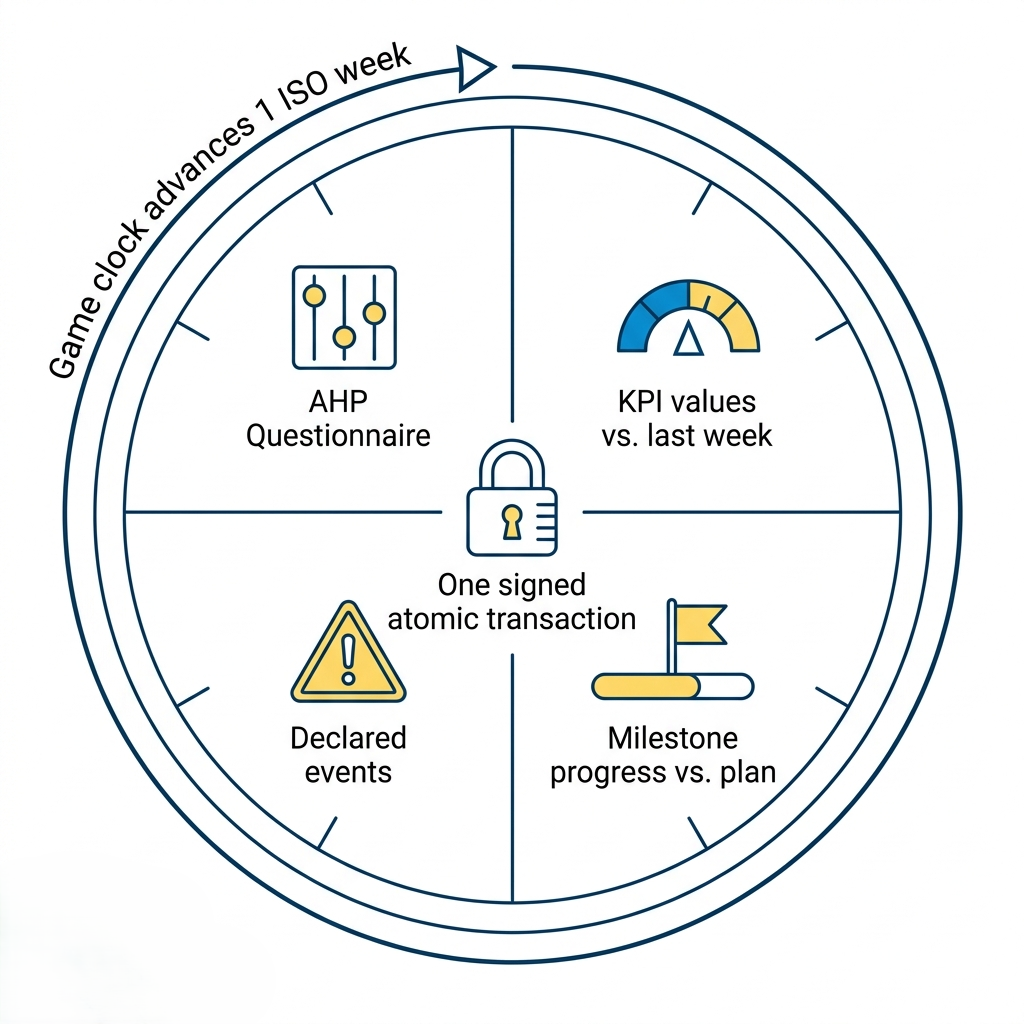
\includegraphics[width=0.85\linewidth]{Images/4.Operations/weekly_cycle.png}
    \caption{The four-section weekly review cycle committed as a single signed transaction.}
    \label{fig:todraw_weekly}
\end{figure}

\begin{figure}[H]
    \centering
    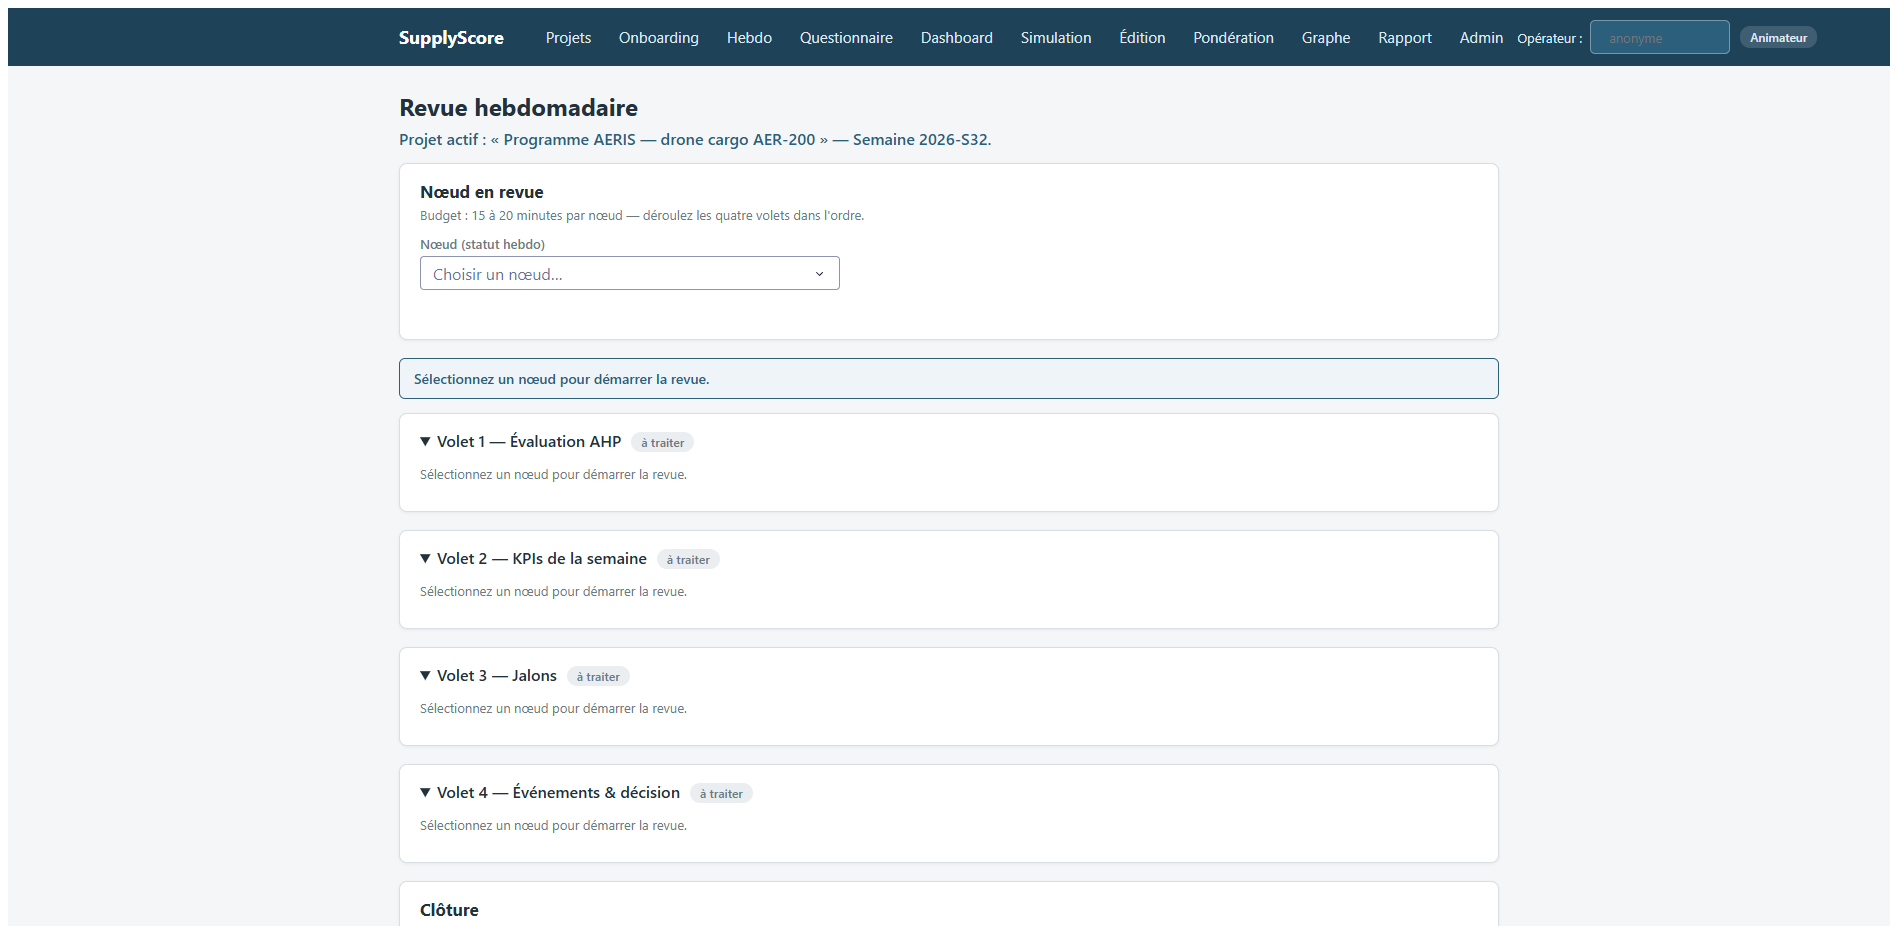
\includegraphics[width=0.85\linewidth]{Images/4.Operations/hebdo.png}
    \caption{Weekly review page: the four sequential sections (AHP, KPIs, milestones, events).}
    \label{fig:hebdo}
\end{figure}

\paragraph{Calibrated Event Engine.}
Rather than asking operators to manually recompute the KPI impact of a disruption, the system exposes a taxonomy of fourteen calibrated event types (\texttt{domain/events.py}), listed in Table~\ref{tab:event_types}, each mapped to one or more KPI updates through one of three calibration operators.

\begin{table}[H]
\centering
\caption{The fourteen calibrated event types.}
\label{tab:event_types}
\small
\begin{tabularx}{\linewidth}{XXX}
\toprule
\texttt{panne\_machine} & \texttt{retard\_fournisseur} & \texttt{greve} \\
\texttt{hausse\_tarif} & \texttt{rupture\_matiere} & \texttt{accident} \\
\texttt{non\_conformite\_qualite} & \texttt{perturbation\_transport} & \texttt{instabilite\_politique} \\
\texttt{cyber\_incident} & \texttt{hausse\_energie} & \texttt{alerte\_financiere\_}\allowbreak\texttt{fournisseur} \\
\texttt{perte\_capacite} & \texttt{pic\_demande} & \\
\bottomrule
\end{tabularx}
\end{table}

The three calibration operators are: a Beta-Bernoulli Bayesian update for failure probabilities,
\begin{equation}
    p_{\text{post}} = \text{clip}\!\left(\frac{p\times n_0 + k}{n_0+n},\, 10^{-4},\, 0.99\right),
    \label{eq:bayes_update}
\end{equation}
with a prior weight $n_0=26$ (roughly six months of weekly observations); an exponential moving average for continuous variables such as OEE, $x_{\text{new}} = (1-\lambda)x_{\text{old}} + \lambda x_{\text{obs}}$ with $\lambda \in [0.3, 0.5]$; and a ratchet (max) update for severity, $s_{\text{new}} = \max(s_{\text{old}}, s_{\text{event}})$. Table~\ref{tab:event_components} defines the shared terms.

\begin{figure}[H]
    \centering
    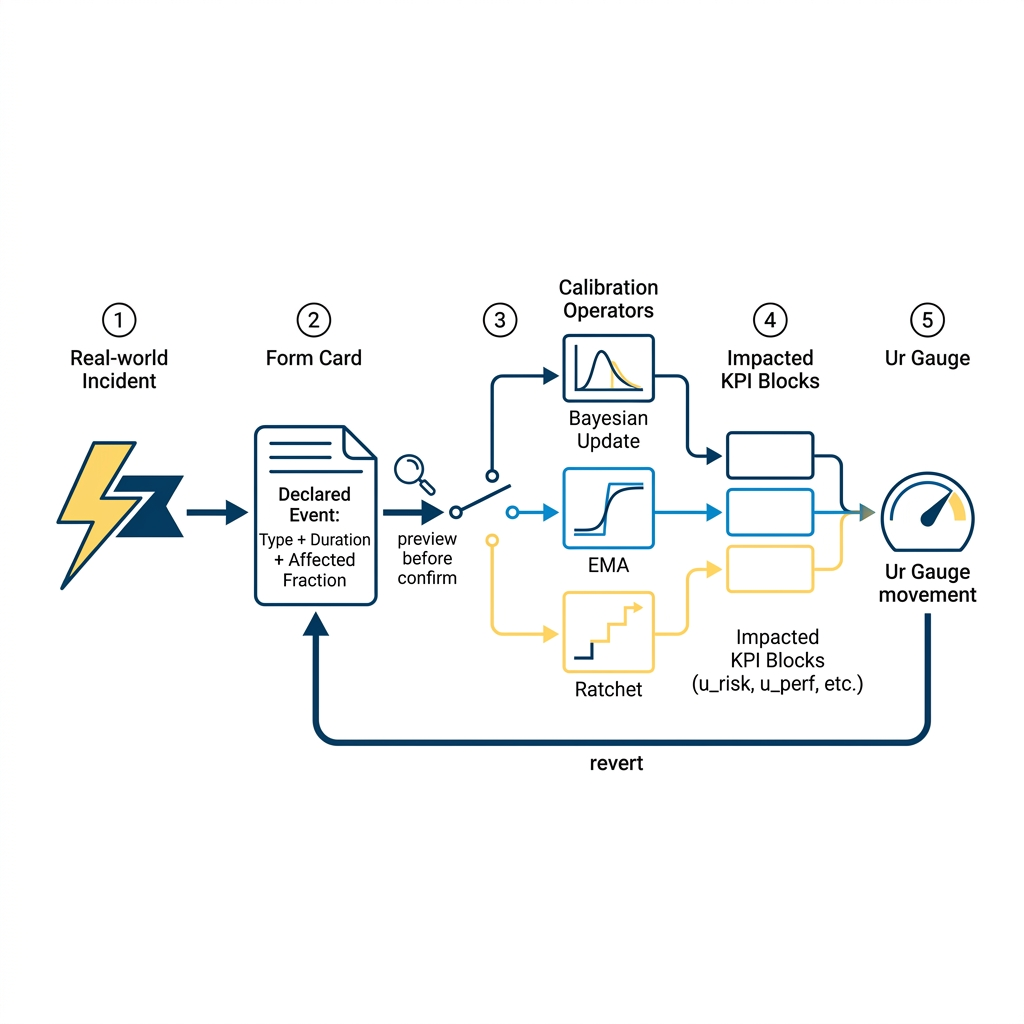
\includegraphics[width=0.85\linewidth]{Images/4.Operations/event_pipeline.png}
    \caption{From a declared event to a calibrated KPI update: the three calibration operators.}
    \label{fig:todraw_events}
\end{figure}

\begin{table}[H]
\centering
\caption{Component definitions for the event calibration operators.}
\label{tab:event_components}
\small
\begin{tabularx}{\linewidth}{llX}
\toprule
\textbf{Component} & \textbf{Type} & \textbf{Description} \\
\midrule
$p_{\text{post}}$ & Dependent variable & Revised failure probability after the event \\
$n_0$ & System parameter & Prior equivalent sample size ($26$, roughly six months) \\
$(k,n)$ & Event input & Equivalent failures/trials implied by the declared event's severity \\
$x_{\text{new}}$ & Dependent variable & Revised continuous KPI (e.g., availability) \\
$\lambda$ & System parameter & EMA reactivity weight, $\in[0.3,0.5]$ \\
\bottomrule
\end{tabularx}
\end{table}

\paragraph{Numerical Example: Strike Event.}
A node declares a \texttt{greve} (strike) lasting $d=24$~hours affecting a fraction $p_f=0.50$ of the workforce. Equivalent lost hours over a 168-hour week: $H_{\text{lost}} = d \times p_f = 12$, so $f_{\text{lost}} = 12/168 \approx 0.0714$ and the observed availability is $A_{\text{obs}} = 1 - 0.0714 \approx 0.9286$. Updating a baseline availability $A_{\text{old}}=0.95$ with EMA reactivity $\lambda=0.5$: $A_{\text{new}} = 0.5(0.95) + 0.5(0.9286) \approx 0.9393$. Risk severity is updated in ratchet mode: $S_{\text{new}} = \max(0.30, 0.50) = 0.50$. Operators can preview the transient impact of a declared event before confirming it, and reverting an event recomputes the baseline KPIs automatically.

The weekly cycle and event engine let coordinators keep the digital twin's KPI state current from structured, auditable inputs rather than free-form edits. This is what makes the resulting urgency history usable as a calibration dataset for the campaign of Section~\ref{sec:serious_game}.

%% ═══════════════════════════════════════════════════════════════════════════
\subsubsection{Explainability, Export, and Operational Hardening}
\label{sec:explain_export}
%% ═══════════════════════════════════════════════════════════════════════════

When the digital twin flags a node, the coordinator's first question is \emph{why}. The last three capabilities of the demonstrator exist to answer that question exactly, to let the data leave the tool, and to make sure nothing is ever lost.

\paragraph{Explainability.}
The per-node explanation page (\texttt{services/explain.py}) answers "why this score?" with exact decompositions, not approximations. Declared urgency splits into one additive contribution per AHP criterion, the same construction as Equation~\ref{eq:ud_local} read term by term:
\begin{equation}
    \kappa_j = w_j\,\frac{s_j-1}{8}, \qquad \sum_j \kappa_j = U_{d,\text{local}},
\end{equation}
so the page can state, for instance, that half of a node's declared urgency comes from the time-window criterion. Local real urgency splits the same way through the logarithm of Equation~\ref{eq:ur_local}: each block contributes $\ell_m = -\omega_m\ln(1-u_m)$, the block shares $c_m = \ell_m / \sum_k \ell_k$ sum to one, and $U_{r,\text{local}} = 1-\exp(-\sum_m \ell_m)$ reconstructs the score exactly. A coordinator can therefore see which block drives a node's urgency, and whether the gap between $U_d$ and $U_r$ is panic or hidden danger (Figure~\ref{fig:ponderation}).

\begin{figure}[H]
    \centering
    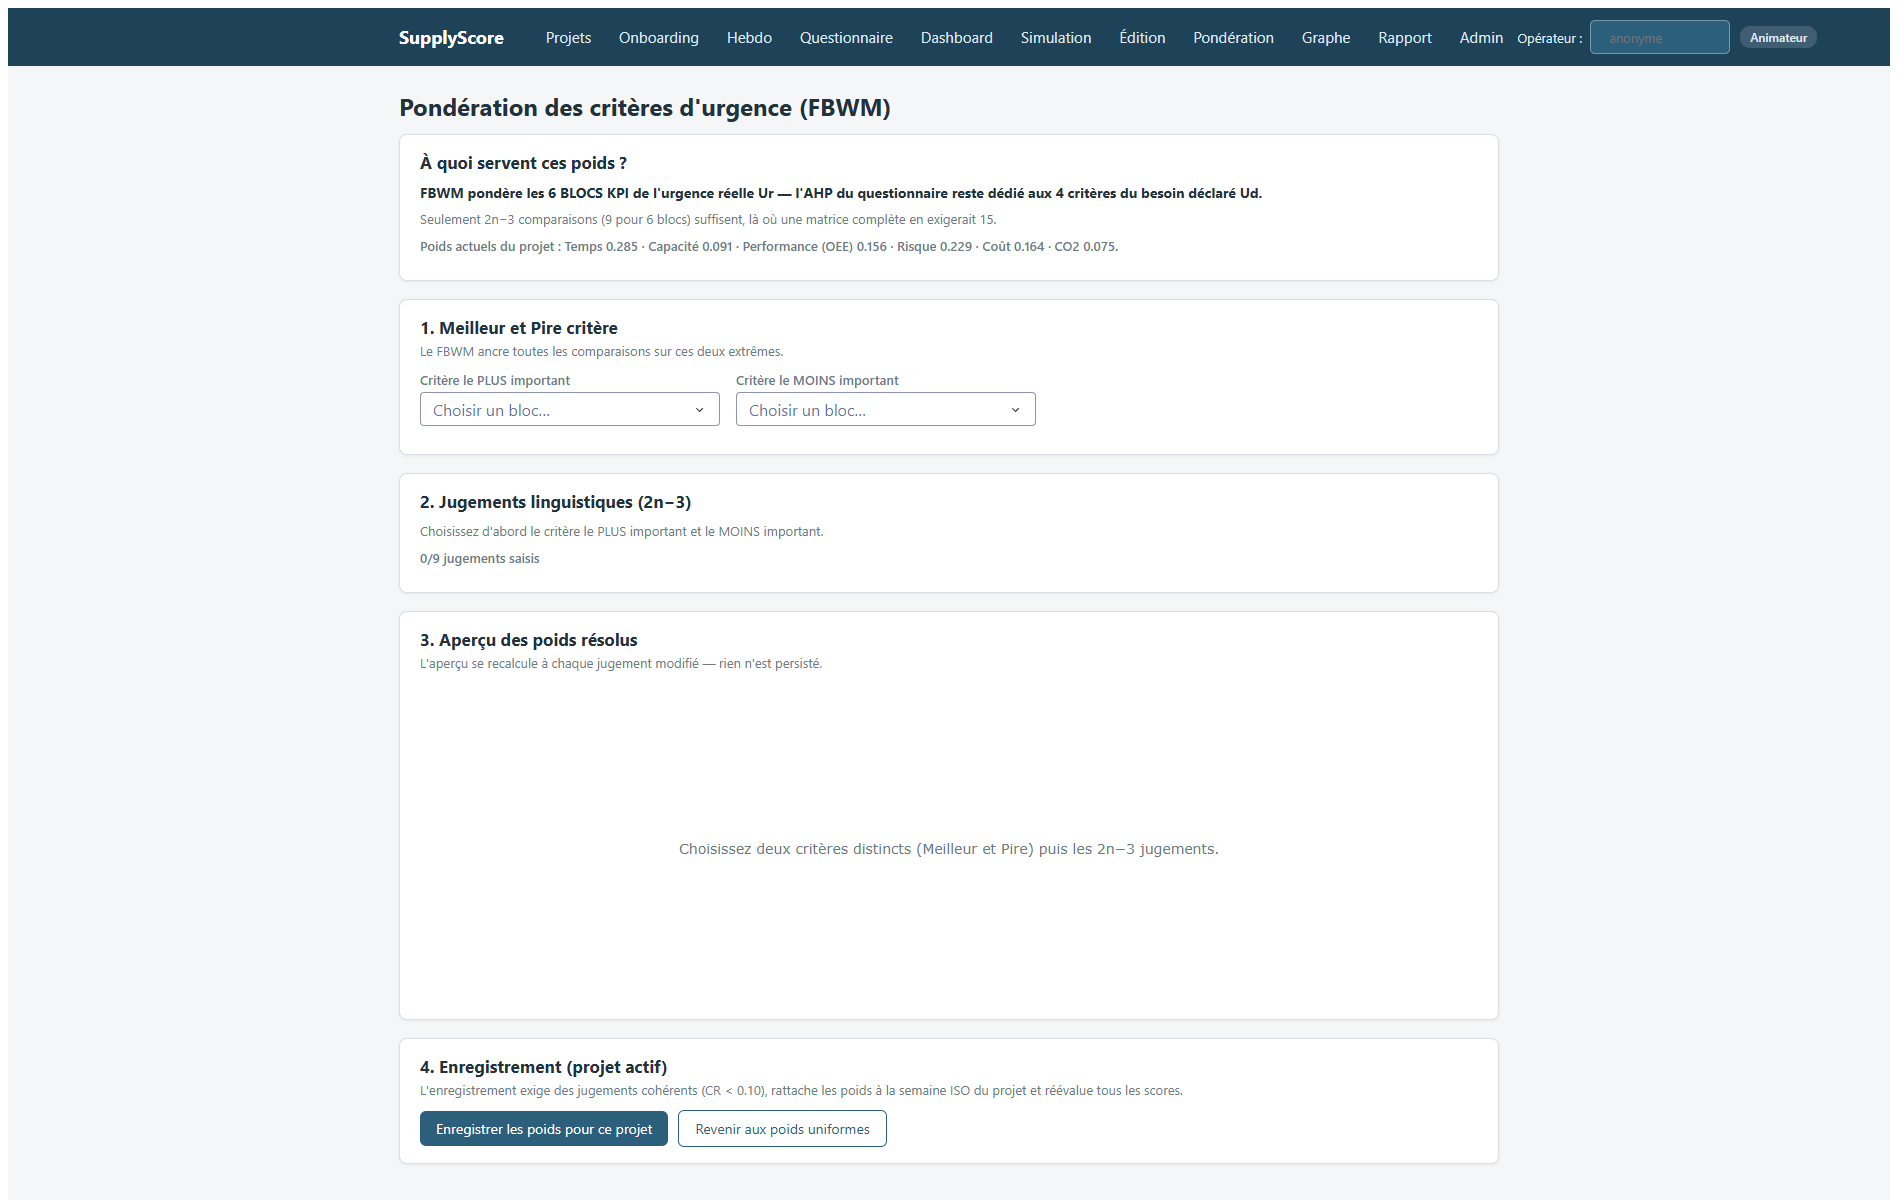
\includegraphics[width=0.85\linewidth]{Images/4.Operations/ponderation.png}
    \caption{Criteria weighting interface (Fuzzy-BWM) feeding the explainability decomposition.}
    \label{fig:ponderation}
\end{figure}

\begin{figure}[H]
    \centering
    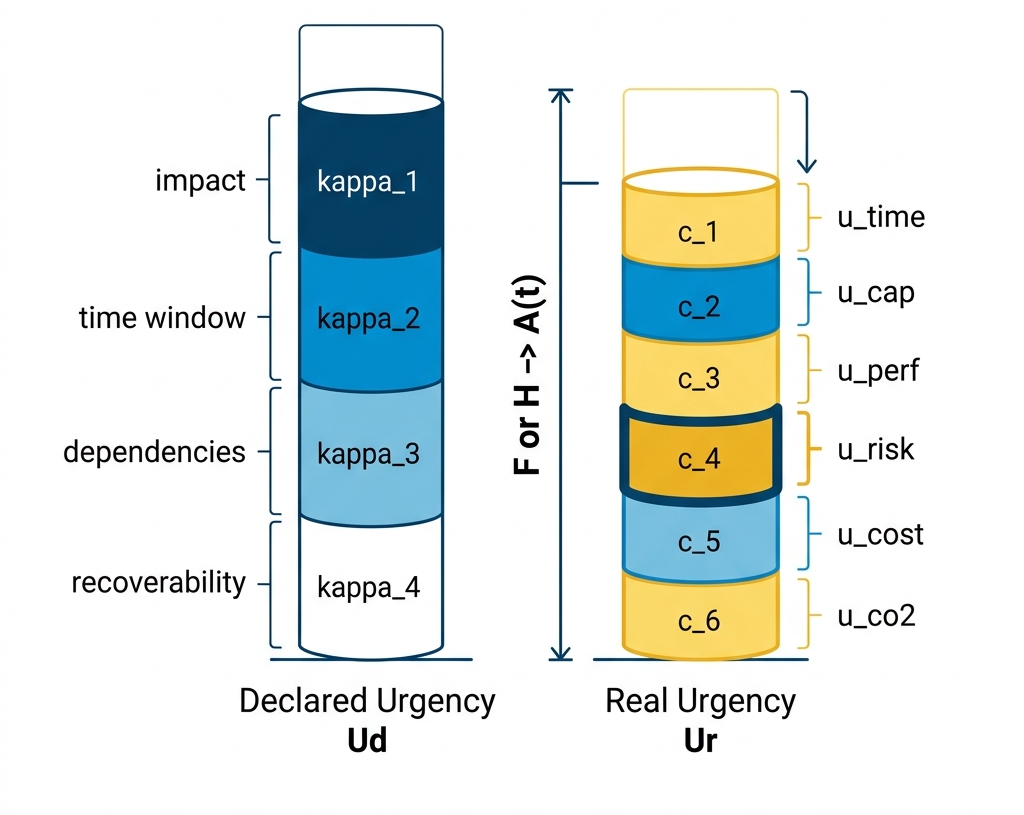
\includegraphics[width=0.85\linewidth]{Images/4.Operations/explainability_waterfall.png}
    \caption{Per-node explainability: exact additive decomposition of $U_d$ and $U_r$.}
    \label{fig:todraw_explain}
\end{figure}

\paragraph{Export.}
One action compiles the global registry and the per-node history into a twelve-worksheet Excel workbook (\texttt{services/exports.py}): project metadata, nodes, arcs, milestones, KPI history, urgency history, assessments, weekly reviews, KPI snapshots, events, decisions, and two audit-log sheets. All timestamps are converted to the coordinator's local timezone. Analyses can therefore run outside the tool, on frozen data, which the validation campaign relies on.

\paragraph{Operational Hardening.}
The persistence layer is SQLite, so data safety is handled explicitly (\texttt{data/}\allowbreak\texttt{backup.py}): Write-Ahead Logging is enabled, an integrity check runs before every backup, and the native \texttt{sqlite3.backup} API copies each database without locking the running application. Automatic backups run every 24 hours with a retention cap of 20 archives, and schema migrations are versioned (Figure~\ref{fig:admin}).

\begin{figure}[H]
    \centering
    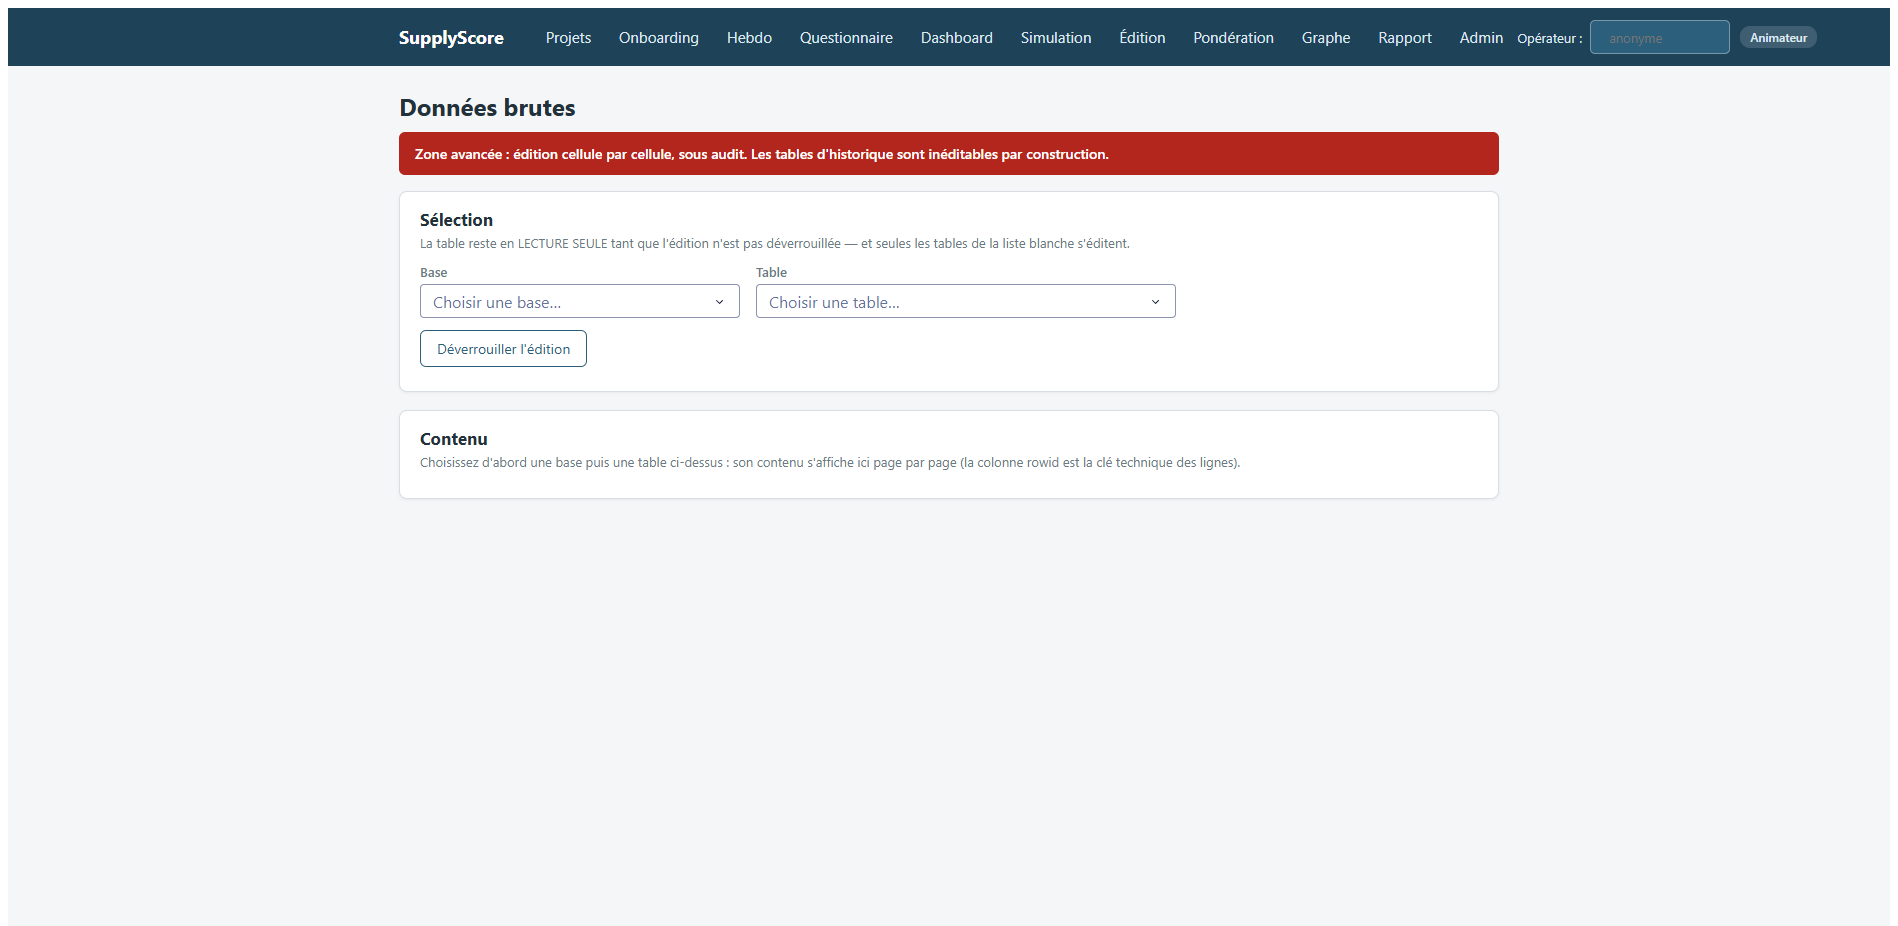
\includegraphics[width=0.85\linewidth]{Images/4.Operations/admin.png}
    \caption{Administration page: database sizes, migration version, and backup controls.}
    \label{fig:admin}
\end{figure}

These three capabilities are not peripheral. They are what make the adequacy score auditable and the digital twin operable outside a development environment, and they are preconditions for the campaign below.

%% ═══════════════════════════════════════════════════════════════════════════
\subsection{Use Case and Validation: The HÉLIOS Serious-Game Campaign}
\label{sec:serious_game}
%% ═══════════════════════════════════════════════════════════════════════════

Everything up to this point establishes that the model is implemented, internally consistent, and tested. What it does not establish is whether the adequacy signal says anything true about real operators facing a real crisis. This section presents the validation campaign built for that purpose: its design, its current state of readiness, and what has been learned from the two checks already run against it. The campaign replays the 2020--2022 semiconductor shortage as a serious game, designed, calibrated through five dry runs, and pre-registered before execution.

\paragraph{Campaign Design.}
The campaign, presented to participants under the cover story \emph{Programme HÉLIOS}, replays the semiconductor crisis over 18 weekly game turns compressed into nine working days (two turns per day, morning and late afternoon). Those 18 playing turns follow an opening turn on which the first declarations are made, so a run is indexed T0 to T18 and every result in this section counts nineteen turns; the two figures describe the same campaign. The supply network has eight nodes, one per consultant, anchored on the real actor types of the crisis (Table~\ref{tab:helios_network}).

\begin{table}[H]
\centering
\caption{The eight HÉLIOS campaign nodes and their real-world anchors.}
\label{tab:helios_network}
\small
\begin{tabularx}{\linewidth}{>{\raggedright\arraybackslash}p{3.1cm} >{\raggedright\arraybackslash}p{2.6cm} c X}
\toprule
\textbf{Node} & \textbf{Role} & \textbf{Rank} & \textbf{Real-world anchor} \\
\midrule
Orbitalys & Satellite prime, final customer & 0 & Fictional satellite programme, contractual delivery pressure \\
AvioSys Int\'egration & Avionics integrator & 1 & Qualified-stock squeeze on avionics tier-1 suppliers \\
\'Electis EMS & Electronics manufacturing services & 2 & EMS plants placed under allocation, 2021 \\
CompoDis Europe & Component distributor & 3 & Distributor allocation and spot-market premiums \\
TransGlobal Fret & Freight operator & 3 & Suez Canal blockage, West Coast port congestion \\
NovaFab Semiconductors & Foundry, expected bottleneck & 4 & Composite of the Texas winter-storm freeze and the Taiwan drought \\
Meridian Semi & Secondary foundry, inert backup arc & 4 & A foundry sold out through 2023: the announced "plan B" that delivers nothing \\
SilPure Materials & Raw wafer supplier & 5 & Roughly 60\% of world wafer supply; polysilicon price roughly tripling in 2021 \\
\bottomrule
\end{tabularx}
\end{table}

\begin{figure}[H]
    \centering
    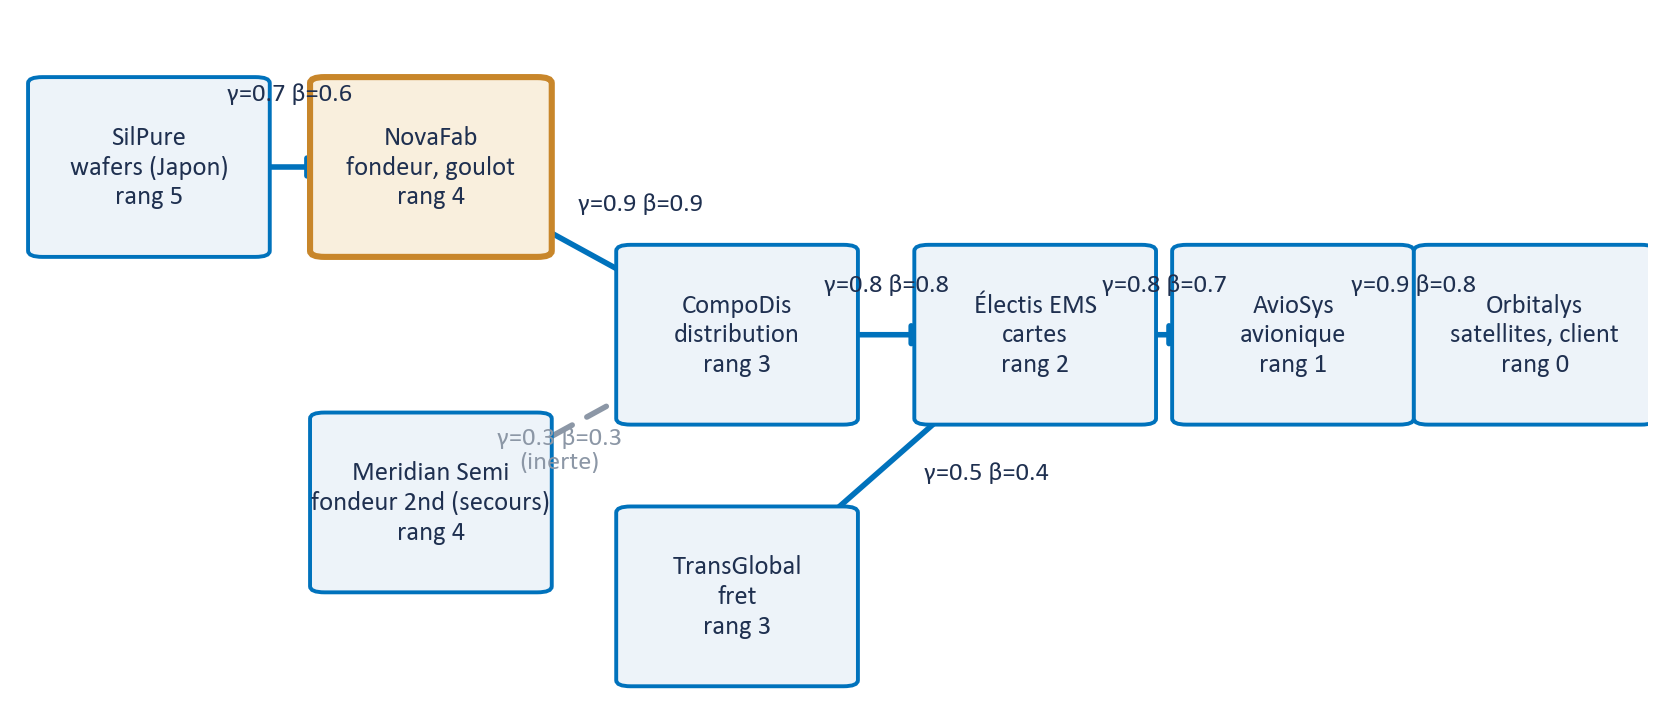
\includegraphics[width=\linewidth]{Images/4.Operations/helios_network_coefficients.png}
    \caption{The HÉLIOS network with its per-arc coefficients: $\gamma$ (downstream demand attenuation) and $\beta$ (upstream risk amplification), and each node's tier rank. NovaFab (rank 4) is the expected bottleneck; the dashed Meridian arc is the inert backup arc of Section~\ref{sec:math_framework}.}
    \label{fig:helios_network_coefficients}
\end{figure}

The eighteen turns follow five acts drawn from the documented chronology of the real crisis: a baseline where early warning signs go unheeded (turns 1--4), a tipping point where a foundry freeze, a competitor fire, and a canal blockage make the crisis visible (turns 5--8), a squeeze where spot prices reach ten to forty times catalogue and no node keeps any margin (turns 9--12), a rupture where a major manufacturer cuts production by roughly 40\%, the bullwhip effect takes hold, and the announced backup foundry turns out to have no spare capacity (turns 13--16), and a slow, partial recovery that measures whether declared urgency lags the physical de-escalation (turns 17--18).

Each act is driven by calibrated engine events whose type, parameters, and timing are taken from that chronology; the twelve events are listed in Table~\ref{tab:helios_events}. One game turn represents one real month, from September 2020 to February 2022, with real durations converted into engine hours at a fixed rate (one real week maps to roughly 38.7 engine hours), so that documented figures such as the twelve-to-twenty-five-week supplier lead times or the six-day canal blockage keep their true magnitude inside an eighteen-turn game.

\begin{table}[H]
\centering
\caption{The twelve calibrated engine events that drive the HÉLIOS crisis, with their real-world anchors.}
\label{tab:helios_events}
\small
\begin{tabularx}{\linewidth}{c >{\raggedright\arraybackslash}p{2.3cm} >{\raggedright\arraybackslash}p{2.9cm} X}
\toprule
\textbf{Turn} & \textbf{Node} & \textbf{Event type} & \textbf{Real-world anchor} \\
\midrule
T3 & NovaFab & Demand spike & Automotive reorders on sold-out slots, Nov.\ 2020 \\
T5 & CompoDis & Supplier delay & Distributor moves to allocation, Jan.\ 2021 \\
T6 & NovaFab & Accident (critical) & Texas winter-storm fab freeze, Feb.\ 2021 \\
T7 & NovaFab & Demand spike & Reorders after a competitor's fab fire, Mar.\ 2021 \\
T7 & TransGlobal & Transport disruption & Suez Canal blockage, six days, Mar.\ 2021 \\
T10 & NovaFab & Material shortage & Taiwan drought, ultrapure-water rationing, Jun.\ 2021 \\
T12 & \'Electis & Capacity loss & Southeast-Asia backend lockdowns, Aug.\ 2021 \\
T12 & TransGlobal & Transport disruption & Shift to saturated air freight, Aug.\ 2021 \\
T13 & CompoDis & Demand spike & Bullwhip over-ordering, Sep.\ 2021 \\
T14 & TransGlobal & Transport disruption & West Coast port congestion, Oct.\ 2021 \\
T14 & CompoDis & Tariff increase & Allocation spot premiums, Oct.\ 2021 \\
T16 & SilPure & Tariff increase & Polysilicon price pass-through, Dec.\ 2021 \\
\bottomrule
\end{tabularx}
\end{table}

One encoding choice is worth noting. The Texas freeze is modelled as a production accident, which triggers the engine's Bayesian revision of the failure probability, a recovery clock, and a severity ratchet, rather than as a capacity loss, which would only reduce storage volume: a hot shutdown of a fabrication line is mechanically closer to the former.

The two urgency signals come from different worlds, which is the point of the design. Real urgency $U_r$ is fed from public time series of the actual crisis (INSEE production and price indices, WSTS worldwide semiconductor billings, and a Kaggle semiconductor-shortage dataset), frozen in a data pack whose SHA-256 hashes were recorded before the first turn. Every third-party dataset is passed through an authenticity check before use: a Kaggle logistics dataset initially considered for the freight node was rejected at this check for the signatures of synthetic training data (pre-computed target columns, GPS coordinates scattered outside the region the dataset claimed to cover, uniformly flat distributions), while the semiconductor-shortage dataset passed (a secular price decline, a genuine 2021 upturn, sectoral employment consistent with official series) and was kept. The rejected dataset is retained in the raw-data folder for audit but is never loaded by the analysis pipeline; the freight node's cost block is instead driven entirely by the calibrated events of Section~\ref{sec:weekly_cycle}. Declared urgency $U_d$ comes from the consultants through the same weekly AHP questionnaire described in Section~\ref{sec:ahp_tool}, under ten minutes per turn, with the consistency gate active.

Two data-provenance rules protect the real-urgency series. First, a single-pilot rule forbids double counting: each KPI field of each node is driven either by a time series or by a calibrated event, never by both, so when an event writes a field on a given turn the series skips that turn. Second, one honest artefact of the real data is kept rather than smoothed away. The INSEE business-failures series falls through 2020 and 2021, under public support schemes, so a failure-rate indicator taken alone would lower external risk exactly while the sector crisis was worsening. Keeping it is the multi-block argument made concrete: a single macroeconomic indicator can tell the opposite of the ground truth, which is why real urgency aggregates six blocks rather than trusting one.

\begin{figure}[H]
    \centering
    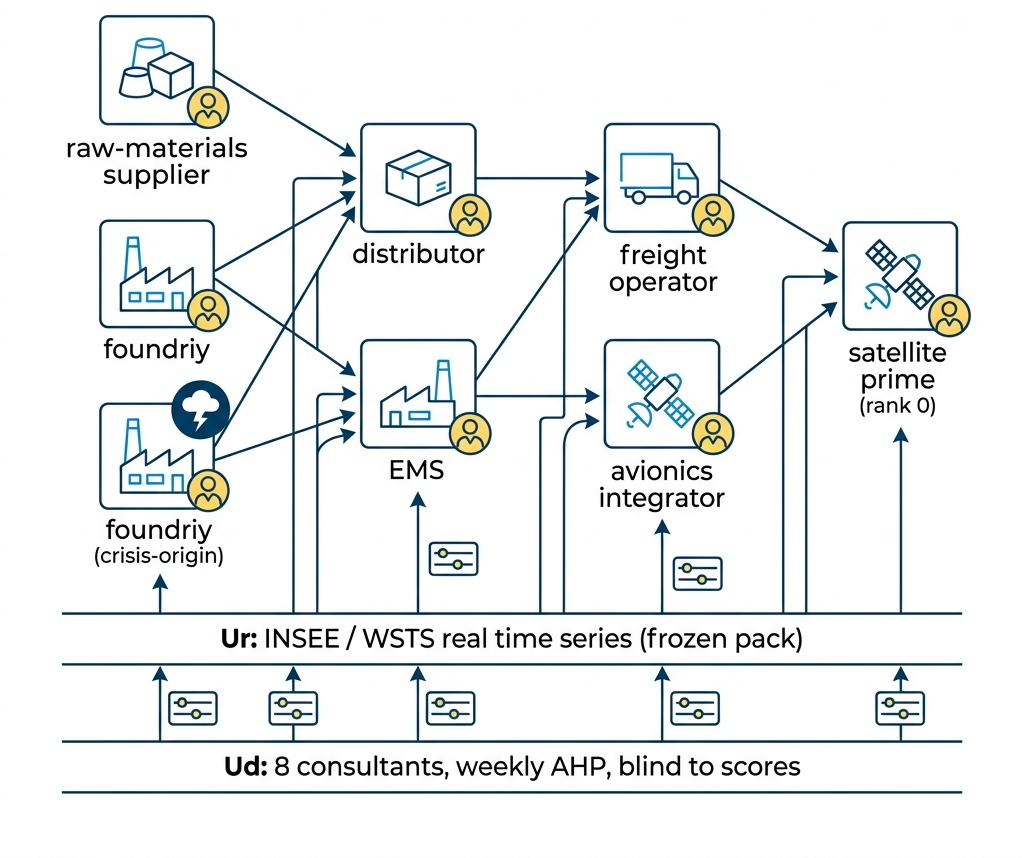
\includegraphics[width=0.85\linewidth]{Images/4.Operations/campaign_network.png}
    \caption{The eight-node HÉLIOS campaign network. The person icon on each node marks the consultant who plays it, feeding $U_d$ through the weekly AHP questionnaire; the lower band shows the public data series that independently feed $U_r$.}
    \label{fig:todraw_campaign}
\end{figure}

\paragraph{Protocol Integrity.}
The experimental protocol was frozen before the first real turn. Consultants see only their own role sheet and the questionnaire page; dashboards and scores stay hidden until the debrief. No discussion between roles is allowed during the campaign. Two placebo sheets, a false de-escalation handed to the avionics integrator at turn 9 and to the wafer supplier at turn 15, control for suggestibility: if a consultant's declared urgency follows the placebo, the measure is reflecting the sheet handed to them rather than a memory of the real crisis. A weak-signal turn (turn 4), where the press mentions a tension with no engine event behind it, measures who reacts to media noise alone. Every deviation from protocol is logged the same day in a campaign journal. Two further safeguards protect internal validity: roles are assigned so that the two most information-heavy nodes, the foundry and the distributor, do not go to the most supply-chain-experienced consultants, keeping a role effect from being confounded with an expertise effect, and at the debrief each consultant is asked at which turn they recognised the real crisis, which turns the main threat to a blind declaration into a measured quantity rather than an uncontrolled one. The hypothesis register is the one of Section~\ref{sec:hypotheses}: H1 to H6, each with a numeric threshold fixed in advance, so that success and failure are defined before the data exists. Any analysis outside that register is labelled exploratory.

\paragraph{Empirical Calibration of the Adequacy Signal.}
The campaign feeds the calibration service (\texttt{services/calibration.py}), which addresses Challenge~3 (Section~\ref{sec:locks}) and hypotheses H2 and H4: does the hidden-risk signal $H$ have predictive value beyond a raw KPI threshold? For each recorded (node, week) pair, the historical hidden risk is compared against negative outcomes observed in a subsequent four-week window (a missed milestone, an abandoned node, or a critical event). The resulting confusion matrix yields precision, recall, and F1:
\begin{equation}
    \text{Precision} = \frac{TP}{TP+FP}, \qquad \text{Recall} = \frac{TP}{TP+FN}, \qquad F1 = \frac{2 \times \text{Precision}\times\text{Recall}}{\text{Precision}+\text{Recall}}.
    \label{eq:calib_metrics}
\end{equation}

\paragraph{Mechanical Validation: The Synthetic Dry Run.}
Before any human data exists, the full campaign mechanics were exercised end to end on a disposable database: five iterations (v1 to v5) calibrated the scenario and eliminated engine artefacts, and the final iteration replayed all nineteen turns (T0 to T18) with synthetic respondents standing in for the eight consultants. This dry run is an engineering check, not a scientific one: the synthetic declared urgency is anchored directly on each node's own local real urgency ($1 + 8 \times U_{r,\text{local}}$, perturbed by a fixed panic, under-report, or neutral bias per role), so it cannot lag its own physical signal, cannot under-report it for long, and cannot over-react to a press event it does not read. Run against the pre-registered tests, the dry run therefore returns not confirmed or not applicable on all six hypotheses by construction (Table~\ref{tab:helios_dryrun}), which is the expected and informative outcome: it confirms that the full pipeline, injection, weekly decay, milestone drift, event calibration, propagation, criticality, snapshotting, and backup, runs correctly under the two-turn-per-day cadence the real campaign requires, and it calibrated the null-baseline detector (a raw threshold $U_{r,\text{local}} \ge 0.5$) at precision $0.16$ and recall $0.27$: the bar the hidden-risk signal must clear in the real campaign to demonstrate added value beyond a raw KPI reading (Challenge~3, Section~\ref{sec:locks}).

\begin{table}[H]
\centering
\caption{Dry-run v5 verdicts on synthetic data: an engineering check, not a hypothesis test.}
\label{tab:helios_dryrun}
\small
\begin{tabularx}{\linewidth}{>{\raggedright\arraybackslash}p{3.4cm} >{\raggedright\arraybackslash}p{2.4cm} X}
\toprule
\textbf{Test} & \textbf{Verdict} & \textbf{Measured value} \\
\midrule
H1 latency & Not confirmed & 1 of 8 nodes at lag $\ge 1$ turn (threshold: 5 of 8) \\
H2 early detection & Not confirmed & $H(\text{NovaFab})$ peaks at $0.070$ on turns 6--12 (threshold: $0.3$) \\
H3 criticality & Not confirmed & NovaFab top-1 on 7 of 10 informative turns, $70\%$ (threshold: $80\%$; saturated turns excluded, Section~\ref{sec:criticality}) \\
H4 predictive validity & Not confirmed & precision $0.00$, recall $0.00$ at $H \ge 0.5$ (threshold: $0.5$; null baseline: precision $0.16$, recall $0.27$) \\
H5 contagion & Not confirmed & non-affected nodes: $\Delta U_d = -0.007$ on press turns vs.\ $+0.031$ on calm turns \\
H6 hysteresis & Not applicable & real urgency shows no measurable decline over the recovery turns, so the comparison is not meaningful \\
\bottomrule
\end{tabularx}
\end{table}

Figure~\ref{fig:helios_dryrun_trajectories} shows why: for every one of the eight nodes, real urgency (solid) and synthetic declared urgency (dashed) track each other closely across the full replay, rather than one lagging or decoupling from the other. That closeness is the visual signature of the circularity described above, not a property the real campaign is expected to reproduce. Table~\ref{tab:helios_trajectories} traces the same propagated real urgency at eight representative turns, showing the crisis propagate through the network broadly as the scenario intends: a slow build in the baseline, the sharp T6--T8 tipping point at NovaFab, TransGlobal, and CompoDis, a saturated network through the squeeze and rupture, and a partial, uneven recovery where NovaFab barely eases while Meridian, hit late by the worldwide demand wave, saturates only at the very end.

\begin{figure}[H]
    \centering
    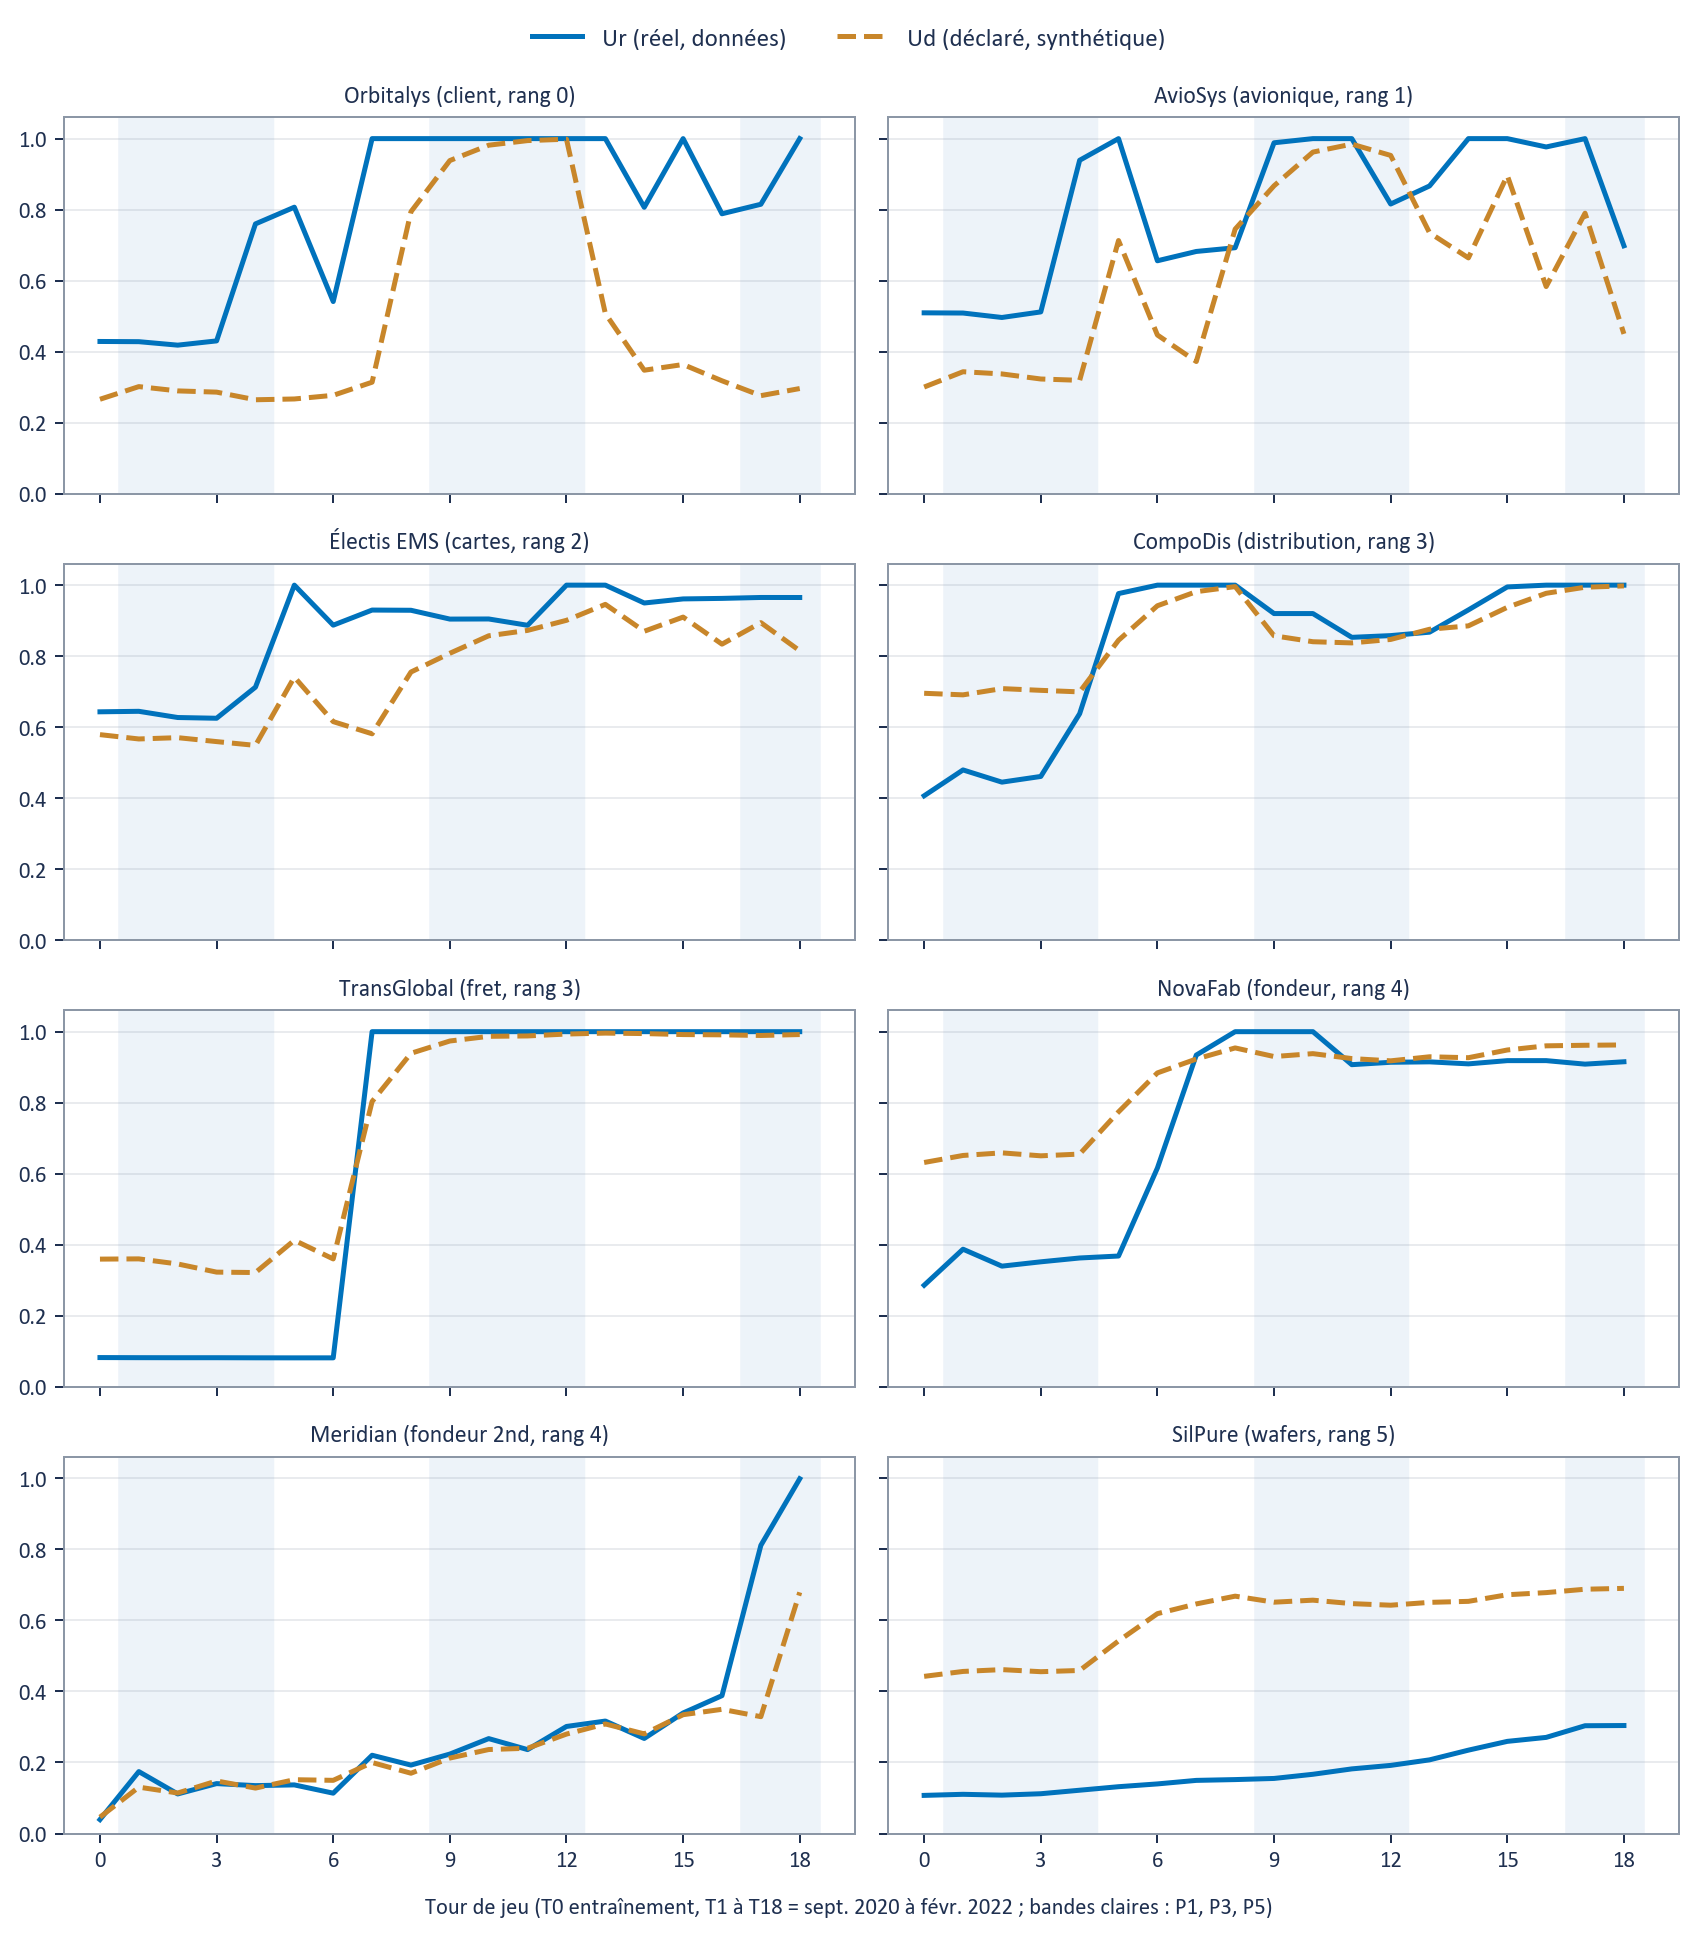
\includegraphics[width=0.85\linewidth]{Images/4.Operations/helios_dryrun_trajectories.png}
    \caption{Real urgency $U_r$ (solid) against synthetic declared urgency $U_d$ (dashed) for all eight nodes across the dry-run v5 replay (T0 to T18, shaded bands mark phases P1, P3, P5). The synthetic $U_d$ follows $U_r$ at every node by construction, which is why H1, H2, H5, and H6 are not interpretable on this run.}
    \label{fig:helios_dryrun_trajectories}
\end{figure}

\begin{table}[H]
\centering
\caption{Propagated real urgency $U_r$ by node across the dry-run v5 replay (selected turns).}
\label{tab:helios_trajectories}
\small
\begin{tabularx}{\linewidth}{l >{\centering\arraybackslash}X >{\centering\arraybackslash}X >{\centering\arraybackslash}X >{\centering\arraybackslash}X >{\centering\arraybackslash}X >{\centering\arraybackslash}X >{\centering\arraybackslash}X >{\centering\arraybackslash}X}
\toprule
\textbf{Node} & T0 & T4 & T6 & T8 & T10 & T13 & T16 & T18 \\
\midrule
Orbitalys & 0.43 & 0.76 & 0.54 & 1.00 & 1.00 & 1.00 & 0.79 & 1.00 \\
AvioSys & 0.51 & 0.94 & 0.66 & 0.69 & 1.00 & 0.87 & 0.98 & 0.70 \\
\'Electis & 0.64 & 0.71 & 0.89 & 0.93 & 0.90 & 1.00 & 0.96 & 0.97 \\
CompoDis & 0.41 & 0.64 & 1.00 & 1.00 & 0.92 & 0.87 & 1.00 & 1.00 \\
TransGlobal & 0.08 & 0.08 & 0.08 & 1.00 & 1.00 & 1.00 & 1.00 & 1.00 \\
NovaFab & 0.29 & 0.36 & 0.62 & 1.00 & 1.00 & 0.92 & 0.92 & 0.92 \\
Meridian & 0.04 & 0.13 & 0.11 & 0.19 & 0.27 & 0.32 & 0.39 & 1.00 \\
SilPure & 0.11 & 0.12 & 0.14 & 0.15 & 0.17 & 0.21 & 0.27 & 0.30 \\
\bottomrule
\end{tabularx}
\end{table}

The confusion matrix behind the H4 row of Table~\ref{tab:helios_dryrun} is given in full in Table~\ref{tab:helios_calibration}, since it is what the real campaign's confusion matrix will be measured against.

\begin{table}[H]
\centering
\caption{Calibration confusion matrix on the dry-run v5 synthetic replay (152 node-turn observations).}
\label{tab:helios_calibration}
\small
\begin{tabularx}{\linewidth}{lX}
\toprule
\textbf{Quantity} & \textbf{Value} \\
\midrule
True positives / false positives (hidden-risk signal, $H \ge 0.5$) & 0 / 5 \\
True negatives / false negatives (hidden-risk signal, $H \ge 0.5$) & 102 / 37 \\
Precision / recall, hidden-risk signal & $0.00$ / $0.00$ \\
Precision / recall, null baseline ($U_{r,\text{local}} \ge 0.5$) & $0.16$ / $0.27$ \\
\bottomrule
\end{tabularx}
\end{table}

\begin{figure}[H]
    \centering
    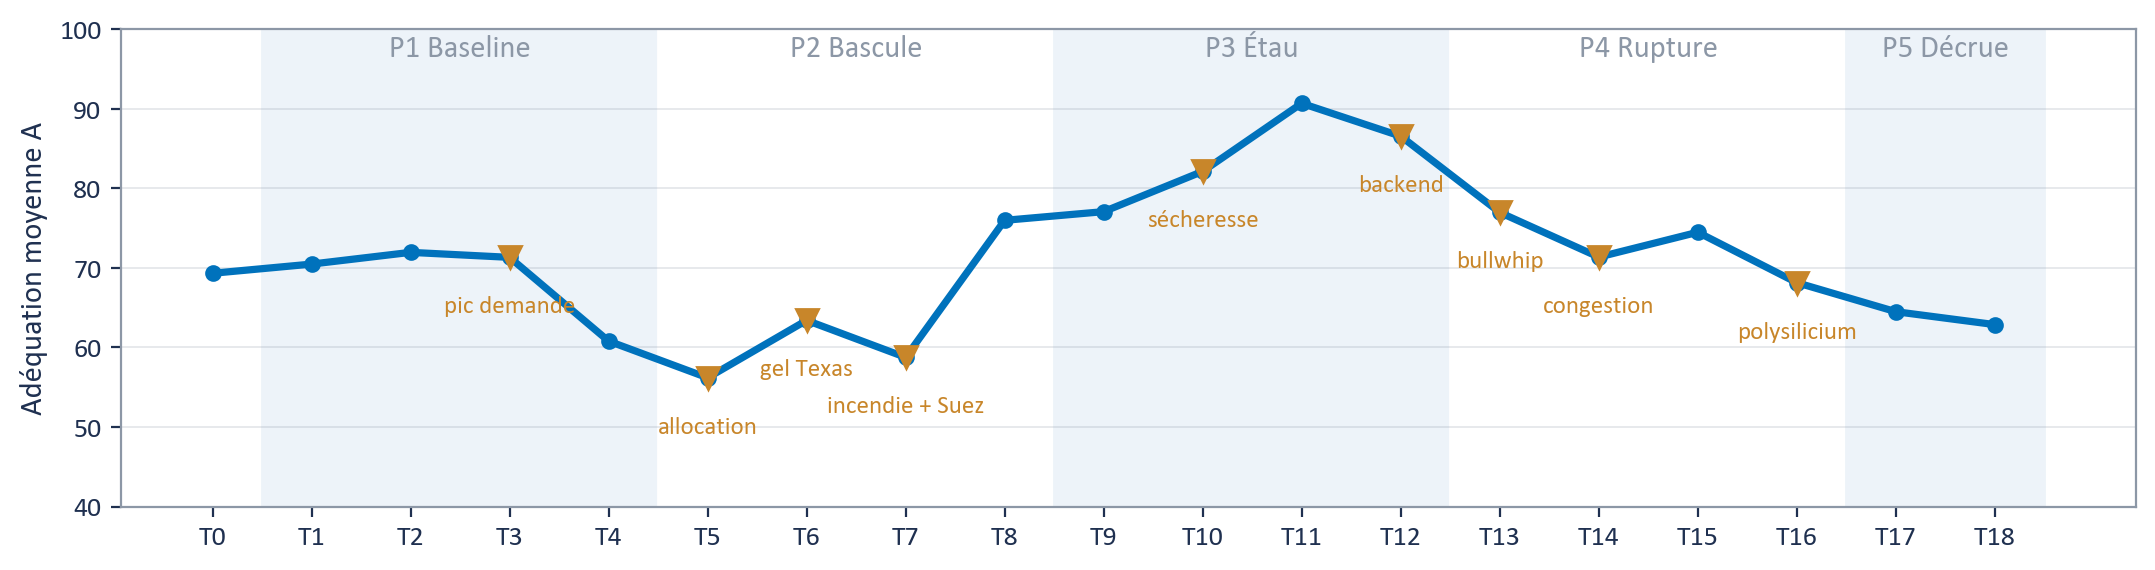
\includegraphics[width=0.85\linewidth]{Images/4.Operations/helios_dryrun_adequacy.png}
    \caption{Network-average adequacy score $A$ across the dry-run v5 replay, annotated with the scenario's calibrated events. The score falls sharply at fast turning points (demand spike, Texas freeze, fire and Suez, drought), then rises through the squeeze (P3) as the saturated network is uniformly tracked by the synthetic $U_d$, before eroding again as the bullwhip and congestion events land.}
    \label{fig:helios_dryrun_adequacy}
\end{figure}

\paragraph{Exploratory Pilot: Eight Isolated Language-Model Agents.}
A second, more informative pilot replaced the fixed-bias synthetic generator with eight isolated large-language-model agents, one per role, each confined to its own role card and turn briefings, with no access to the other roles, the dashboard, or future turns, the same anti-lookahead discipline required of the real consultants. Each agent read its briefing in character and answered the real AHP tool of Section~\ref{sec:ahp_tool}, pairwise comparisons and severity scores through the production consistency-ratio code. Unlike the synthetic dry run, this pilot exercised the full production pipeline rather than a standalone computation: campaign setup, turn injection, and questionnaire submission all ran through the same weekly-cycle service (\texttt{services/orchestrator.py}) that a browser-based consultant reaches, closing on the same live dashboard built for the real campaign. This pilot is exploratory: it was not part of the pre-registered protocol, and a single language-model instance per role has no statistical standing as a substitute for eight independent human judges. Table~\ref{tab:helios_llm_pilot} gives its verdicts on the same six pre-registered tests.

\begin{table}[H]
\centering
\caption{LLM-pilot verdicts: eight isolated language-model agents replaying the real AHP questionnaire through the production pipeline (exploratory, not pre-registered).}
\label{tab:helios_llm_pilot}
\small
\begin{tabularx}{\linewidth}{>{\raggedright\arraybackslash}p{3.4cm} >{\raggedright\arraybackslash}p{2.4cm} X}
\toprule
\textbf{Test} & \textbf{Verdict} & \textbf{Measured value} \\
\midrule
H1 latency & Not confirmed & 3 of 8 nodes at lag $\ge 1$ turn (threshold: 5 of 8) \\
H2 early detection & Not confirmed & $H(\text{NovaFab})$ peaks at $0.017$ on turns 6--12 (threshold: $0.3$) \\
H3 criticality & Not confirmed & NovaFab top-1 on 7 of 10 informative turns, $70\%$ (threshold: $80\%$; identical to the dry run, a $U_d$-independent test) \\
H4 predictive validity & Not confirmed & precision $0.00$, recall $0.00$ at $H \ge 0.5$ ($TP=0$, $FP=2$, $TN=105$, $FN=37$) \\
H5 contagion & Confirmed & non-affected nodes: $\Delta U_d = +0.079$ on press turns vs.\ $+0.005$ on calm turns \\
H6 hysteresis & Not applicable & real urgency shows no measurable decline over the recovery turns \\
\bottomrule
\end{tabularx}
\end{table}

Two results stand out. The urgency-contagion hypothesis (H5) is confirmed: declared urgency of non-affected nodes rises by $0.079$ on press-event turns against $0.005$ on calm turns, matching the pre-registered direction and ordering. The latency hypothesis (H1) moves from 1 of 8 nodes on the synthetic dry run to 3 of 8 nodes at a lag of one turn or more, closer to, but still short of, the pre-registered threshold of 5. Both results are a first sign of a non-circular declared-urgency signal: a reasoning-based judge, unlike the dry run's formula, can in principle lag or amplify the physical signal instead of tracking it by construction. H4 stays not confirmed, but for a specific and informative reason: these agents read their briefing carefully and declared urgency close to what the briefing in fact described, so their $U_d$ tracks $U_r$ too closely to leave the gap that $H$ is built to catch, an even tighter tracking than the fixed-bias dry run ($H(\text{NovaFab})$ peaks at $0.017$ against $0.070$). H3 is unchanged from the dry run because it depends only on the network's real-urgency criticality ranking, not on $U_d$ at all. H6 stays not applicable for the same reason as the dry run: real urgency shows no measurable decline over the recovery turns. Taken together, this pilot motivates, without yet establishing, the idea that a genuinely reasoning-based declared-urgency signal can decouple from the physical signal in the way the model's hypotheses predict, and it sharpens rather than removes the case for the real campaign: only a human's imperfect, potentially under-reporting perception of a crisis, not a careful reader's, can put H4 to a fair test.

\paragraph{The Pilot's Final Application State.}
The pilot did not just produce six hypothesis verdicts: it left behind a live SupplyScore project, reloadable in the same dashboard a coordinator would use in production. Read directly from that project after the eighteenth turn, the network-average adequacy is $65.5$, four of the eight nodes carry a hidden-risk reading above $0.1$, one carries a false-urgency reading above $0.1$, and the single worst-scoring node by a wide margin is Orbitalys at $A=15.3$; Table~\ref{tab:llm_pilot_snapshot} lists the full per-node snapshot.

\begin{table}[H]
\centering
\caption{Final per-node snapshot of the LLM pilot's SupplyScore project, read directly from the application after turn 18.}
\label{tab:llm_pilot_snapshot}
\small
\begin{tabularx}{\linewidth}{l >{\centering\arraybackslash}X >{\centering\arraybackslash}X >{\centering\arraybackslash}X >{\centering\arraybackslash}X >{\centering\arraybackslash}X}
\toprule
\textbf{Node} & $U_d$ & $U_r$ & $A$ & $F$ & $H$ \\
\midrule
Orbitalys & 0.409 & 1.000 & 15.3 & 0.000 & 0.591 \\
AvioSys Intégration & 0.727 & 0.698 & 95.2 & 0.029 & 0.000 \\
Électis EMS & 0.914 & 0.965 & 82.9 & 0.000 & 0.052 \\
CompoDis Europe & 0.882 & 1.000 & 67.5 & 0.000 & 0.118 \\
TransGlobal Fret & 0.819 & 1.000 & 56.0 & 0.000 & 0.181 \\
Meridian Semi & 0.841 & 0.998 & 60.1 & 0.000 & 0.157 \\
NovaFab Semiconductors & 0.912 & 0.915 & 98.5 & 0.000 & 0.003 \\
SilPure Materials & 0.876 & 0.304 & 48.9 & 0.572 & 0.000 \\
\bottomrule
\end{tabularx}
\end{table}

Orbitalys' own explanation page traces the chain from a single scripted event to this score without manual computation. Its next milestone, the HÉLIOS-1 delivery, had slipped past its deadline by turn 18, which forces $u_{\text{time}}$ to $1$ under the rule of Table~\ref{tab:ur_blocks}; with the node's real urgency already saturated by this cause alone, the explanation page attributes the whole of it to the local block, none to the upstream network. The agent playing Orbitalys, meanwhile, declared $U_d=0.41$. The resulting hidden risk $H=[U_r-U_d]_+=0.59$ is penalised through Equation~\ref{eq:penalty} at $2.25\times0.59^{0.88}=1.42$, giving $A=100\times(e^{-1.42}-e^{-2.25})/(1-e^{-2.25})=15.3$, the same number the dashboard reports, reconstructed term by term by the explainability page of Section~\ref{sec:explain_export} rather than by hand. The network-wide PROMETHEE~II ranking (Section~\ref{sec:fbwm_promethee}) places NovaFab and Orbitalys at the top of the priority list ($\phi=+0.220$ and $+0.215$), the expected bottleneck and the node its own missed milestone makes most urgent, though the same ranking carries a caveat the tool raises on its own: on this run, the time and performance blocks are perfectly correlated ($\rho=1.00$), the composite-indicator risk already flagged in Section~\ref{subsec:mcdm}.

\paragraph{The Executed Campaign: Two Arms on a Frozen Scenario.}
The campaign has since been executed in its agent version, with eight isolated language-model declarants in place of the eight consultants, over nineteen turns on the frozen scenario. Two arms were run. In the control arm each declarant sees only its own role card and turn briefing and declares blind. In the treatment arm the same declarants are additionally shown the system's own predictive analysis of their node before declaring, and record whether it influenced them. Because the scenario is frozen, the two arms carry numerically identical forecasts, which was verified on all 72 shared predictions, so any behavioural difference belongs to the act of displaying them and not to a different prediction.

The result on the prediction layer is negative and precise. Scored against the outcome definition the calibration service itself applies, the four-week forecast reaches an area under the ROC curve of $0.485$ with a confidence interval containing $0.5$, and a Brier skill of $-3.36$ against a forecaster that simply announces the base rate. Twenty-one forecasts announced a mean probability of $0.948$ and none was followed by the predicted outcome, while the 74 forecasts announcing a mean of $0.070$ were followed by an adverse outcome $8.1\%$ of the time. The model is close to right where it announces low probabilities and wrong where it announces high ones, which is the profile that isolates a single defective channel rather than a broken formulation. That channel is the time block: across all twenty-one confident forecasts the four-week probability and the milestone-miss probability never differ by more than $0.020$.

\paragraph{The Cause, and the Repair That Followed.}
The cause is structural rather than statistical. The time block computes milestone risk from a lead-time distribution against a deadline, while the calibrated event engine writes to capacity, cost and failure probability and to no quantity on the time axis. The evidence is a count that depends on no scoring choice: across the whole campaign, eight nodes and 41 indicator snapshots each, the accumulated-delay field the block would need was written a non-zero value exactly zero times. The block cannot respond to a disruption, and because it drives the entire confident tail, neither can the forecast.

That defect was then repaired and the campaign rescored on the identical frozen forecasts. The obvious repair, making the events write a lead-time impact, was implemented first and measured to be wrong: a quantity routed into the lead time is multiplied by the fraction of work remaining, so a shock attenuates in proportion to how close a milestone is to completion and vanishes on the milestones nearest their deadline, which are exactly those where a warning has value. On the foundry node the four-week probability fell from $0.846$ to $0.000$ on a milestone that was in fact missed. Lost production time is additive, so the completion estimate was rewritten as $C = t + (1-p)L + R$, with $p$ the declared progress, $L$ the lead time and $R$ the time already lost, identically in the three independent estimators the system carries for that quantity. Five families of capacity-halting event now accumulate into $R$; loss of storage capacity deliberately does not, since it removes space rather than production hours.

Two further defects were exposed by the first. The forecast rollout drew the lead time at random but treated the declared progress as an exact value, which made the milestone probability return exactly zero or exactly one in $85\%$ of cases; progress is now drawn per replicate with a spread widened node by node in proportion to that node's own measured hidden risk, so the adequacy measurement feeds the forecast. And indicator coverage on the campaign database was $25.6\%$, with 24 of the 42 indicators empty on every node and only three of the six urgency blocks contributing anything, which is a diagnosis about the data rather than the mathematics. Completing the indicators from public figures of the real shortage raised coverage to $49.1\%$, activated all six blocks, and exposed one model bug that had been undetectable while the database was empty: a per-node recovery capability was being read as production time already lost.

Table~\ref{tab:bst_reparation} gives the rescoring. It is stated against a target that judges a milestone by the deadline the node originally committed to rather than by whatever deadline the milestone currently carries, because a replanning is itself the admission of a slip and a truth in which re-dating erases the miss scores the forecast against the outcome it was built to warn about.

\begin{table}[H]
\centering
\caption{The frozen campaign rescored after repair, on the same 120 forecasts.}
\label{tab:bst_reparation}
\small
\begin{tabularx}{\linewidth}{c *{4}{>{\centering\arraybackslash}X}}
\toprule
\textbf{Horizon} & \textbf{Brier skill before} & \textbf{Brier skill after} &
\textbf{AUC before} & \textbf{AUC after} \\
\midrule
1 week  & $-1.278$ & $-0.687$ & 0.736 & 0.729 \\
2 weeks & $-0.690$ & $-0.367$ & 0.636 & 0.634 \\
3 weeks & $-0.654$ & $-0.286$ & 0.641 & 0.602 \\
4 weeks & $-0.553$ & $-0.216$ & 0.654 & 0.584 \\
\bottomrule
\end{tabularx}
\end{table}

The calibration deficit is roughly halved at every horizon. Three things must be said against that. The Brier skill remains negative, so the forecast is still worse calibrated than announcing the base rate. The movements in the area under the ROC curve are not interpretable, since with 26 positive observations the interval on the four-week figure runs from $0.21$ to $0.87$ and contains every value in its row. And the milestone probability is still degenerate in $71.7\%$ of cases against $85.0\%$ before.

\paragraph{A Hypothesis That Became Measurable Again.}
The saturation collapse of the criticality index (Section~\ref{sec:criticality}) forced hypothesis H3 to be judged on ten turns of nineteen, the other nine being saturated and therefore uninformative. With the log-survival key those turns can be ordered again, and H3 was re-measured. On the repaired run, applying the old criterion alone gives 10 informative turns and NovaFab top-1 on 9 of them; adding the $\Delta \ell$ key gives 17 informative turns and NovaFab top-1 on 16 of them, a share of $94\%$ against the pre-registered threshold of $80\%$. Under the old criterion held fixed, the frozen campaign gave $70\%$ and the repaired one gives $90\%$, so the completion of the indicators moves the figure as well as the new key does.

This is stated as an exploratory re-measurement and not as a verdict, for a reason that should be explicit: the pre-registered H3 was measured on the frozen campaign with the code as it then stood, and a hypothesis re-run on a changed model no longer tests what the register asked. Two things changed at once here, the ranking key and the model with its data, and only the first is cleanly isolated, by comparing the two criteria on the same run. What can be claimed is narrower and still useful: the degeneracy that made nearly half the campaign unreadable is largely gone, and the quantity H3 tests now sits above its threshold on the repaired system.


\paragraph{Behaviour: What Happens When the Forecast Is Displayed.}
The treatment arm produced a second result that was not sought. For the first four turns the forecast is hidden and all eight declarants record no influence. At the turn it first becomes visible, all eight record one, and the direction is entirely one-sided: five revised their declared urgency downward and three had their existing assessment confirmed, with no upward revision anywhere. The scenario's single critical event lands two turns later, on the foundry node. Over the full campaign the balance is close to even, 15 upward revisions against 16 downward, so the one-sided effect belongs to first contact rather than being a permanent bias. Two things make this more than a curiosity: the forecast being displayed comes from the layer whose confident predictions never materialised and whose time block is blind to the very shock about to arrive, and it is displayed as a numeric probability with a confidence interval, which is the format the automation-bias literature identifies as increasing reliance. The system was presenting an unfounded reassurance in its most persuasive available form.

\paragraph{A Closed Loop on the Repaired System.}
A third arm was then run on the repaired system, in which the same eight declarants no longer only declared but also selected actions from a fixed catalogue applied to the chain by the mutation service and recorded in the intervention journal: promote a backup arc, replan a milestone, expedite a shipment, raise capacity, revise a declaration, or do nothing. One hundred and fifty-two declarations were recorded over nineteen turns with no unresolved consistency failure.

Its headline figure flatters the tool and should not be used. Six of eleven milestones were missed in the frozen scenario and none was left unfinished in the closed loop, which reads as six saved. Judged against the original commitments it is not: five of eleven milestones were met on their original date in the frozen run and five of eleven in the closed loop. The loop changed which milestone was met and not how many. One was genuinely saved, an electronics series delivered on its original date that had slipped in the frozen truth; four late deliveries became replannings announced in advance rather than slips discovered at the deadline, which has value to a customer without being a save; and one milestone was replanned that would have been met, which is the measurable cost of over-reaction. With eleven milestones neither the benefit nor the cost is statistically established, and both are stated as facts of one campaign rather than as results. What does carry is that the causal chain the first campaign showed to be broken now closes: where the foundry declarant of the control arm recorded that the tool was holding a low position through a widely reported crisis and took no action, the repaired run moved the same node's four-week probability from $0.088$ to $0.214$ at the shock turn and the declarant replanned its milestone.

\paragraph{Current Status and Remaining Steps.}
The campaign protocol is frozen, the data pack is hashed, all six operating scripts are delivered, and three arms have been executed with language-model declarants. The human campaign, the only run able to decide the six pre-registered hypotheses as they were written, has not taken place: role assignment, the half-day kickoff, the nine working days of paired turns, and the reveal debrief remain to be executed, and they should now be run against the repaired model rather than against the defective one. The results above are therefore reported for a population of reasoning agents and not for human operators, which is the principal limit on every behavioural statement in this section. Section~\ref{sec:Conclusions} states this as the immediate next step of the programme, together with what the recorded results will feed back into.
